\documentclass[]{article}
\usepackage{fullpage}
\usepackage[authoryear]{natbib}
\usepackage{setspace}
    \doublespacing
\usepackage{hyperref}
\hypersetup{
    colorlinks,
    citecolor=black,
    filecolor=black,
    linkcolor=cyan,
    urlcolor=cyan
}
\usepackage{amssymb,amsmath}
\usepackage{bm}
\usepackage{dcolumn}
\usepackage{booktabs}
\usepackage{url}
\usepackage{tikz}
\usepackage{todonotes}
\usepackage[utf8]{inputenc}
\usepackage{graphicx}
\usepackage{longtable}
\usepackage{todonotes}
\usepackage{lscape}
\usepackage{float}
\usepackage[margins]{trackchanges}
\addeditor{MH}
\addeditor{CG}
\usepackage{subfig}
\captionsetup{belowskip=12pt,aboveskip=4pt}

\usepackage{footmisc}
\renewcommand{\footnotelayout}{\doublespacing}



\title{The Measurement of Real-Time Perceptions of Financial Stress: Implications for Political Economy Models of Crisis}



\author{Christopher Gandrud \\ \emph{City University London} \\ \emph{Hertie School of Governance}\footnote{Please contact Christopher Gandrud
(\href{mailto:christopher.gandrud@city.ac.uk}{\nolinkurl{christopher.gandrud@city.ac.uk}}).
Thank you to Nicole Rae Baerg, Vincent Arel-Bundock, Ronen Palan, Stefano Pagliari, David Singer, and participants at the 2015 American Political Science Association Annual Conference, the 2015 International Political Economy Society Conference, and City University London for helpful comments. We also thank Sahil Deo and Christian Franz for early research assistance. Our research is generously supported by the Deutsche Forschungsgemeinschaft. All data and replication material can be found at:
\url{https://github.com/christophergandrud/EIUCrisesMeasure}.}
\and
Mark Hallerberg \\ \emph{Hertie School of Governance}}

\begin{document}

\maketitle

\begin{center}
    \textbf{Working Draft. Comments welcome.}
\end{center}


\begin{abstract}

Responding to financial market disruptions is a defining challenge for policymakers and central topic of political research. However, established measures of financial conditions have significant shortcomings. Binary crisis indicators \cite[e.g.][]{laeven2013} are constructed \emph{post hoc}, biasing them towards severe events. This has important theoretical implications--studies using these variables cannot differentiate between periods of calm and periods where governments effectively addressed emerging trouble. Continuous indicators capture quantities whose importance, measurement, and reporting varies significantly across countries. We use a kernel principal component analysis (KPCA) of \emph{Economist} monthly country reports to create a continuous measure of real-time perceived stress severity. Not only does it more accurately capture a key concept political scientists often want to study, but it can be used to test theories that were previously difficult to test. We also demonstrate how KPCA can be used to summarize large corpora of texts into continuous indicators.

\end{abstract}


\textbf{Word count:} 8,191

\clearpage

Why and how do politicians respond to financial market stress? What are the political consequences of extreme stress, i.e. crisis? When do policymakers successfully diffuse financial stress so that there is no financial crisis in the first place? What political conditions enable this behavior? These questions have attracted considerable attention at least since the 2007-2010 crisis and earlier Latin American and Asian financial crises in the 1980s and 1990s.

However, most research on these topics lacks a crucial variable: a continuous indicator of the level of financial market stress that policymakers perceived in real-time. To understand why politicians made a given choice in response to financial market stress, we need a measure of the conditions that they perceived at the time.

To measure financial market distress originating in the banking sector,\footnote{It is important to note that there are a number of different types of financial crisis. \cite{reinhartRogoff2011} argue that there are four types of crisis that fit under the definition of ``financial crisis''. Some countries fall into inflation crises when prices get out of control. Others experience currency crises where a government cannot establish a floor on the international price of its domestically printed money. Banking crises occur when large parts of the domestic banking sector are insolvent.  Finally, sovereign debt crises emerge when governments have difficulty repaying their creditors. \citeauthor{reinhartRogoff2011} note that all these crises have debt accumulation at their root.

While all of these types of events are important for political scientists to understand, in this paper, we focus on periods with disruption originating or strongly effecting banking markets. We do widen the scope, however, to consider financial markets more broadly, not just the banking sector. The collapse of the insurance company AIG in 2008 is a reminder that the definition of a ``financial firm'' extends beyond banks to include firms that are active on financial markets.} the literature has relied on a number of binary--e.g. \cite{Reinhart2009,ReinhartRog2010} and Laeven and Valencia \citeyearpar[and their predecessors]{laeven2013}--and continuous--e.g. \cite{Lepetit2013} and \cite{Andrianova2015}--measures of financial market stress. The binary crisis measures--where 1 typically signifies a ``crisis'' and 0 otherwise--are constructed \textit{post hoc} and so tend to be biased towards severe crises and away from circumstances where governments effectively responded to emerging trouble. As such, they suffer from clear selection bias. Additionally, \textit{post hoc} measures do not necessarily capture conditions as they were perceived at the time. Being dichotomous indicators, they do not indicate crisis severity or how it varies over time. The binary measures also often use \textit{ad hoc} methods of determining when stress has returned to normal. Continuous measures of financial market stress are less common in the political economy literature, but they also suffer from other problems. They capture quantities whose importance, measurement, and reporting varies significantly across countries and over time.

To overcome these issues, we develop a new continuous measure of real-time perceptions of financial market stress. We create this variable using a kernel principal component analysis (KPCA) of detailed qualitative data, namely monthly \emph{Economist Intelligence Unit} (EIU) reports. We call it the EIU Perceptions of Financial Market Stress Index--\emph{FinStress} for short.

Being an indicator of perceived and real-time stress, rather than \emph{post hoc} evaluations of policy decisions in response to market events, FinStress provides a much more relevant indicator for understanding policymakers' decision-making process. FinStress is continuous, so it is not \textit{a priori} weighted towards periods with particular government responses and does not select out episodes of stress where policymakers successfully avoided extreme disruption. Because it is a summary of qualitative assessments of qualitative and quantitative data in country-time context, it is comparable across countries. This is crucial for accurately estimating the effect that financial market stress has on policy actions. The measure also has considerably better coverage than previous quantitative measures of stress over the time period for which it is currently available.

FinStress also enables new political research possibilities. For example, as a continuous rather than binary measure of stress, FinStress could be used to examine what policies are effective at preventing or reducing extreme stress and importantly what political conditions are conducive to implementing these policies. As a comparable monthly indicator, FinStress could also be used to test new hypotheses that rely on sub-annual data.\footnote{For example, \cite{gandrud_pepinsky2015} use FinStress variance across quarters to test a new hypothesis that ``good'' economic conditions make it difficult for policymakers to predict crises.}

Not only do we create a measure of financial market stress, but we contribute to the wider political science literature by showing how KPCA can be used to summarize vast quantities of qualitative texts into continuous cross-sectional time-series indicators.

\section{Previous Measures and Use in Research}\label{motivation}

\subsection{Binary measures}

Researchers studying the political economy of crises mostly rely on two data sources of cross-country information on when a country is facing a financial crisis--\cite{Reinhart2009,ReinhartRog2010} and Laeven and Valencia \citeyearpar[and their predecessors]{laeven2013}.

Reinhart and Rogoff \citeyearpar[10]{Reinhart2009,ReinhartRog2010} classify countries as being in crisis when they experience at least one type of event: (1) one or more bank runs, closure, merger, or public sector takeover and/or (2) closure, merger, takeover or large-scale public assistance of an important financial institution that marks the start of a string of similar events. Laeven and Valencia \citeyearpar[228]{laeven2013} take a similar approach that nonetheless explicitly emphasizes public interventions. They classify a country-year as in crisis when there is both significant distress in the banking system and policymakers respond to the distress with significant interventions.\footnote{They define `significant intervention' as at least three of the following six policies being used: deposit freezes/banking holidays, significant bank nationalizations, bank restructuring gross costs, extensive liquidity support, significant guarantees, and significant asset purchases \cite[][229]{laeven2013}. Please see the Online Appendix for a full list of the criteria these data sets use to code a given country-year as being in a crisis.}

These indicators have been widely employed in the literature and so have been critical variables for studying the political economy of financial crises. \cite{Fielding2015} and \cite{Herrera2014} use Laeven and Valencia's indicator as a dependent variable when attempting to understand how capital flow bonanzas affect the probability of crises occurring. Similarly, \cite{Danielsson2015} use \cite{Reinhart2009} to understand how stock price volatility predicts crises. \cite{Keefer2007} and \cite{Rosas2006,Rosas2009} used earlier versions of the \cite{laeven2013} data set to identify periods of crisis and to argue that electoral competitiveness affected policy responses, as well as in Keefer's case, the overall costs of the crisis to taxpayers. \cite{reischmann2015} uses the Laeven and Valencia measure to examine electoral effects on ``creative public budget accounting'', proposing that creative accounting occurs at a higher volume during crises. \cite{seiferling2015} use the Laeven and Valencia measure to find that the composition of government assets is different in crisis periods for advanced and emerging economy countries, such that advanced countries make more loans and purchase more equities in insolvent firms. \cite{ha2015} find using the Laeven and Valencia data set that developing country governments respond to crises with fiscal and monetary tightening, but that this is moderated by political constraints--veto players--, left-wing ideology, and upcoming elections. \cite{Gandrud2013,Gandrud2014} and \cite{Kleibl2013} combine the two data sources to understand how financial regulatory structures are changed in response to crises. \cite{broz2013} takes a similar approach of integrating the data sets to find a ``partisan financial cycle'' where right-leaning pro-market governments implement policies that create economic booms, but also lead to crises. Voters then elect left-leaning governments to clean up afterwards. \cite{CrespoTenorio2014}, \cite{Chwieroth2013}, and \cite{Pepinsky2012} use the data sets in their research on the political effects of crises. \cite{CrespoTenorio2014} find that incumbents in countries with open capital markets are more likely to survive a crisis in power than incumbents in countries with closed capital markets.\footnote{For an additional review of the literature see \cite[1-3]{GandrudHallerberg2015}, as well as tables \ref{LitRevTable2} and \ref{LitRevTable} in the Online Appendix.}

The binary crisis indicators have a number of strong characteristics. They come from detailed comparative work that identifies some key features of crises, including estimated fiscal costs for a large number of countries. Yet, there are a number of problems with these indicators for studying political behaviour. Crucially, crises are identified \emph{post hoc} by researchers who know what happened after the fact. Financial market stress that policymakers successfully address, thus preventing a major visible crisis, is not included. Similarly, stress that a government temporarily dampens through unsustainable policy measures, only to flare up later, is not recorded. The measures are dichotomous and so do not give any indication of how severe crises were. Crises rarely have uniform intensity over their course. Binary indicators do not allow us to understand intensity of a crisis over time.  Having an annual dichotomous measure also means that measurement errors--incorrectly timing the start or end of a crisis--can strongly bias econometric model estimates. All of these factors make it difficult to study why and how politicians respond to financial market stress.

There are also practical coding issues for scholars who use these measures. There are large inconsistencies between the timing of crises in the \cite{laeven2013} and \cite{Reinhart2009} data sets \citep{Chaudron2014}. For example, Japan is labeled as having a crisis between 1997 and 2001 by the former, but between 1992 and 1997 by the latter. Furthermore, \cite{GandrudHallerberg2015} find that there are significant differences in crisis timing between different versions of the \cite{laeven2013} data. While the measures use fairly precise definitions of when a crisis started, reasons for dating the end of a crisis are either unstated as in the case of \cite{Reinhart2009} or are \emph{ad hoc}. Laeven and Valencia \citeyearpar[footnote 19]{laeven2013} determine that a crisis has concluded when real GDP and real credit growth are positive for two years, or five years have elapsed from the crisis start year.

\subsection{Continuous measures}

There are alternative approaches that not only aim to code extreme stress, but also continuous variations in stress severity over time.

\cite{Romer2015} attempt to address many of the problems in the \cite{Reinhart2009} and \cite{laeven2013} data sets. To address the dichotomous variable concern, they use a 16 point scale of the cost of credit intermediation, which provides an indication of stress intensity. They code 24 countries using information from the OECD's semi-annual \emph{Economic Outlook} reports from 1967 to 2007. Their continuous measure gives an indication of distress intensity. Relying on contemporaneous reports allows for the construction of a real-time measure of credit market distress and addresses potential problems with \emph{ex post} coding. Researchers can examine policy choices that head off trouble or, conversely, prolong and perhaps worsen difficulties.

While their approach is an important improvement over previous work, it is limited in a number of ways. First, their data sources means they are necessarily confined to the relatively small sample of OECD countries. Second, because their measure is laborious and time consuming to create and update, even if there were a more encompassing corpus of texts than the OECD \emph{Economic Outlook}, actually applying the method would be costly. Third, relying on human coders may introduce well-known problems of inter-coder reliability and unreproducibility \citep{Minhas2015}.

Another approach is to measure stress and crisis using nationally aggregated quantitative accounting data. The finance literature relies on a statistical quantity known as bank Z-Scores. The concept was originally developed to assess firm solvency \citep[see][]{roy1952}. In the banking context, it is often used to measure national financial system fragility, which allows researchers to examine how banking system structures and policies affect the probability of financial system difficulties \citep[e.g.][]{beck2013bank,vcihak2010islamic,laeven2009bank,uhde2009}. Though there are various ways to calculate this measure \citep[73]{Lepetit2013}, in general bank accounting information--assets, equity, and return on assets--is used to create an inverse measure of the probability that a country's banking system will become ``insolvent''.

Similarly, the CAMELS system uses accounting data to rate bank soundness. The CAMELS indicators include a bank's capital adequacy, asset quality, management capacity, earnings, the liquidity of its assets, and its sensitivity to market risks. \cite{Andrianova2015} gathered individual bank data from the Bankscope service on these quantities for 128 countries, created annual national aggregates, and released the components in a ``database on financial fragility''.

Research looking at longer time spans has been limited by what data is available at the bank-level for measuring banking system health. \cite{Danielsson2015}, for example, examine the Minskian \citeyearpar{Minsky1982} hypothesis that stable conditions in the present induce increased risk-taking behaviour and thus crises in the future with annual stock market volatility. This data allows them to cover a period of 211 years. It seems plausible that stock market volatility is positively associated with broader financial market volatility. Nonetheless, it is well understood in political economy \citep[seminally][]{hall2001introduction} that equity markets are a subset of banking and credit markets overall and that their importance for financing banks and the ``real'' economy varies considerably by country and over time.

There have been a number of further innovations to the measurement of banking system stability using quantitative data. Though they make interesting contributions to measuring financial market stress, these indicators have not been used in applied research as frequently as Z-Scores or CAMELS components. Building on \cite{vonHagen2007}, \cite{Jing2015} develop an index of money market pressure based on changes in short-term interest rates and stocks of central bank reserves. Problematically for the study of policy responses, it assumes that central banks use the same reaction function to increase demand for liquidity. \cite{Rosas2009dltm} developed a dynamic latent trait model of banking system distress. His measure relies on nationally reported data to the IMF's International Financial Statistics (IFS).

Most simply, we could perhaps use individual indicators from the IFS or the broader Global Financial Development Database \citep[GFDD,][]{worldbank2015},\footnote{Many IFS indicators are also reported in the GFDD.} such as the provision of private sector credit by deposit banks as an indicator of credit conditions or non-performing loan ratios as an indicator of bank balance sheet health. However, there are a number of issues with these indicators.

First, the importance of each individual measure for the health of a financial system varies depending on the context. For example, government-run financial institutions may be important providers and recipients of credit, rather than deposit banks.

Second, how these indicators are measured can vary significantly across countries. Many of the GFDD indicators, for example, have a note attached that ``due to differences in national accounting, taxation, and supervisory regimes, these data are not strictly comparable across countries''.

Third, \cite{GandrudCopHal2015} show that national reporting to the IFS and GFDD is highly uneven across countries and time. As such, they indicate that decisions to report data to the IFS and GFDD could be endogenous to economic and political events, complicating attempts to use these data to measure financial market conditions to study political economy phenomena. \cite{cghBruegel2015} find that reporting on credit market conditions declined significantly in the European Union in the lead up to and during the crisis beginning in 2007. Further indicating the pervasiveness of the missingness problem with quantitative data, \cite{Andrianova2015} extensively discuss problems of missingness in their privately gathered database on financial fragility and caution users of the database about the effects it might have on their analysis.

Fourth, as \cite{KayserLeininger2015} show, people make decisions based on contemporaneously available information, but researchers attempting to understand their behaviour often use data that has been significantly updated after the fact. Similar to the binary crisis indicators' \textit{post hoc} measurement problem, using revised IFS and GFDD data gives an inaccurate impression of the conditions that politicians believed they faced at the time.

\section{Creating the FinStress Index}

We overcome many of the problems noted above by using a new approach to estimate real-time perceptions of financial market stress through machine classification of \emph{Economist Intelligence Unit} reports.\footnote{See \url{http://www.eiu.com/}. Accessed May 2015.} Our method uses kernel principle component analysis \citep{Scholkopf1998,lodhi2002,Spirling2012} of monthly country reports from the \emph{Economist Intelligence Unit} to create a monthly index for more than 180 countries from 2003 through 2011.\footnote{Our approach is broadly similar to \cite{Minhas2015} who use a supervised machine learning approach called support vector machines and United States State Department Country Reports on Human Rights Practices to classify countries according to dichotomous regime types. Our work is distinct in that KPCA of EIU reports allows us to develop a continuous measure of perceived financial market stress. Also, their supervised learning approach assumes that countries have been well classified by previous indicators, which they use to train the model. As discussed above, we are not confident that this is the case for financial crisis. Therefore, we use the unsupervised KPCA approach to establish new estimates.}

\subsection{Why the EIU?}\label{why-the-eiu}

The EIU compiles real-time, third-party qualitative assessments of financial market conditions within country-year contexts. Reports are released monthly or, for a small subset of countries, quarterly. These reports contain perceptions of both present and future economic conditions. They are also an important channel through which this information is disseminated to public and private actors in many countries. Together, the reports create a large corpus--more than 20,000 texts--of reports for more than 180 countries over the period 1997-2011, although, due to issues of format comparability we concentrate on data from 2003. In contrast, the OECD \emph{Economic Outlook} used by \cite{Romer2015} provides comparable reports for a very small number of wealthy countries on a bi-annual basis. As such, the EIU is preferable for creating a cross-country indicator of perceived financial market stress.

\subsection{Summarising financial market stress in the
EIU}\label{summarizing-financial-market-stress-in-the-eiu}

Our aim is to create an index that classifies financial conditions on a continuous more-stressed/less-stressed spectrum for as many country-months as possible. Therefore, we need an efficient way to summarize the vast quantity of information in the EIU reports. To do this we first collected and processed the EIU texts. We then used kernel principal component analysis to place the texts onto a financial market stress spectrum. We rescaled the raw spectrum to ease interpretation.

\paragraph{Text selection}\label{text-selection}

EIU reports assess many economic sectors within a country,
not just the financial sector.
Our first step was to select the portions of the EIU texts that contained relevant information about countries' financial systems. We automatically collected and parsed the reports from their original HTML format. We then extracted the portions of the texts--headers and paragraphs--that contained at least one of a number of keywords concerning financial markets.\footnote{The
  keywords included: \emph{bail-out}, \emph{bailout}, \emph{balance
  sheet}, \emph{balance-sheet}, \emph{bank}, \emph{banks},
  \emph{banking}, \emph{credit}, \emph{crunch}, \emph{default},
  \emph{finance}, \emph{financial}, \emph{lend}, \emph{loan},
  \emph{squeeze}. These keywords are adapted
  from those used by \cite{Romer2015} and are intended to
  select passages that discuss credit market conditions. Note that a small number of the words, primarily \emph{bank} and \emph{financial} are by far the most selective.} Due to a significant change in the reports formatted in 2003, we selected only texts from 2003 in order to maintain comparability across the time-series. The texts from 2003 follow the same format and style and contain directly comparable assessments of economic conditions across the globe over a significant time span.\footnote{We also pre-processed the selected texts using standard techniques \citep[see][]{Grimmer2013}. This involved removing common English words, such as `was' and `its'. The `stopword' list we used to do this was from \cite{dhillon:modha:mlj01}. We stemmed the words so that different variants of the same word are represented by a common `stem'. This allowed us to work with a more manageable number of kernels. We removed extra white space between the words, as well as punctuation and numbers. Finally, we dropped texts that included very few words (less than six). In practice, including these texts hindered the estimation of the KPCA model. All pre-processing was done using the \texttt{tm} package \citep{tm2015} in R \citep{R-cite}.}

\paragraph{Kernel Principal Component
Analysis}\label{kernel-principal-component-analysis}

Texts are frequently summarized using unordered `bags-of-words'
approaches that are analysed to find, for example, clusters of topics within speeches or clusters of speeches around topics are common results from these methods \citep[for a review see][]{Grimmer2013}. We would like to preserve word order in our texts. Many financial terms such as `credit growth' and `borrowing costs' have different interpretations depending on the adjectives that modify them; consider, for example, `slowing credit growth' vs. `expanding credit growth' or `falling borrowing costs' vs. `increasing borrowing costs'. Likewise, adjectives can have very different implications for describing market conditions depending on the nouns that they modify;  For example, `increasing' can indicate worsening conditions as in `increasing non-performing loans' or improving conditions as in `increasing lending'.  A bags-of-words approach that treated each word as having meaning as an individual unit, rather than having meaning in ordered associations with other words, would not adequately capture commonly used and radically different meanings in the EIU documents.

In order to address these issues we use kernel principal component analysis. This method was developed by \cite{Scholkopf1998} and \cite{lodhi2002}. \cite{Spirling2012} introduced it into political science. He used it to summarize changing trends in treaties between the US government and Native American groups. KPCA allows us to extract structure from our likely high-dimensional EIU corpus while preserving word order \cite[6531--6537]{Zhang2010}.

Our unit of analysis is a sub-string kernel: a short sequence of letters\footnote{The kernels are similar to n-grams though they do not need to be complete words. Following \cite{Spirling2012}, we used kernels with a length of five, i.e.~those that are five letters long. See also \cite{lodhi2002} who demonstrate that in English string lengths between four and seven are often optimal.} that can be shared within and across words. Thus we can distinguish between two simple documents with the stemmed strings `slow credit' and `expand credit'. They share the five character kernels `credi' and `redit', but differ on `slowc' and `pandc', among others. Using \cite{lodhi2002} we can summarize the similarity of these documents with the frequency distribution of five-length strings that they have in common--in this case one--standardized by document length. We can find these pairs for all of the documents in our corpus to create a kernel matrix. Finally, we can scale the documents using principal component analysis.\footnote{We conducted KPCA with the \texttt{kpca} function from the R package \textbf{kernlab} \citep{kerblabCite}.}

\paragraph{Dimensionality}\label{dimensionality}

To determine the number of dimensions that best describe the data, we conducted a scree test, the results of which are shown in Figure \ref{scree_plot}. There is a clear `elbow' in the plot at component two. This suggests that the first component explains the most variation in the data. In the rest of the article we focus on the first dimension as the main dimension summarizing financial market stress. We examined a number of the other dimensions. However, these noticeably did not closely correspond to our priors about financial market stress based on previous indicators. Below we detail how the first component corresponds to our expectations of a valid measure of financial market stress.

It is important to note two simple transformations we conducted on the raw results to create the final FinStress Index. First, we rescaled it so that it would be between zero and one.\footnote{\(\frac{x - \mathrm{min}(\bm{X})}{\mathrm{max}(\bm{X}) - \mathrm{min}(\bm{X})}\),
  where \(\bm{X}\) is the vector of the first principal component and
  \(x\) is an individual value from this vector.} This eases
interpretation. Second, we smoothed the results by taking a two period--usually two months--moving average.

\begin{figure}
    \caption{Assessing Model Fit: Eigenvalues for Kernel Principal Components}
    \label{scree_plot}
    \begin{center}
        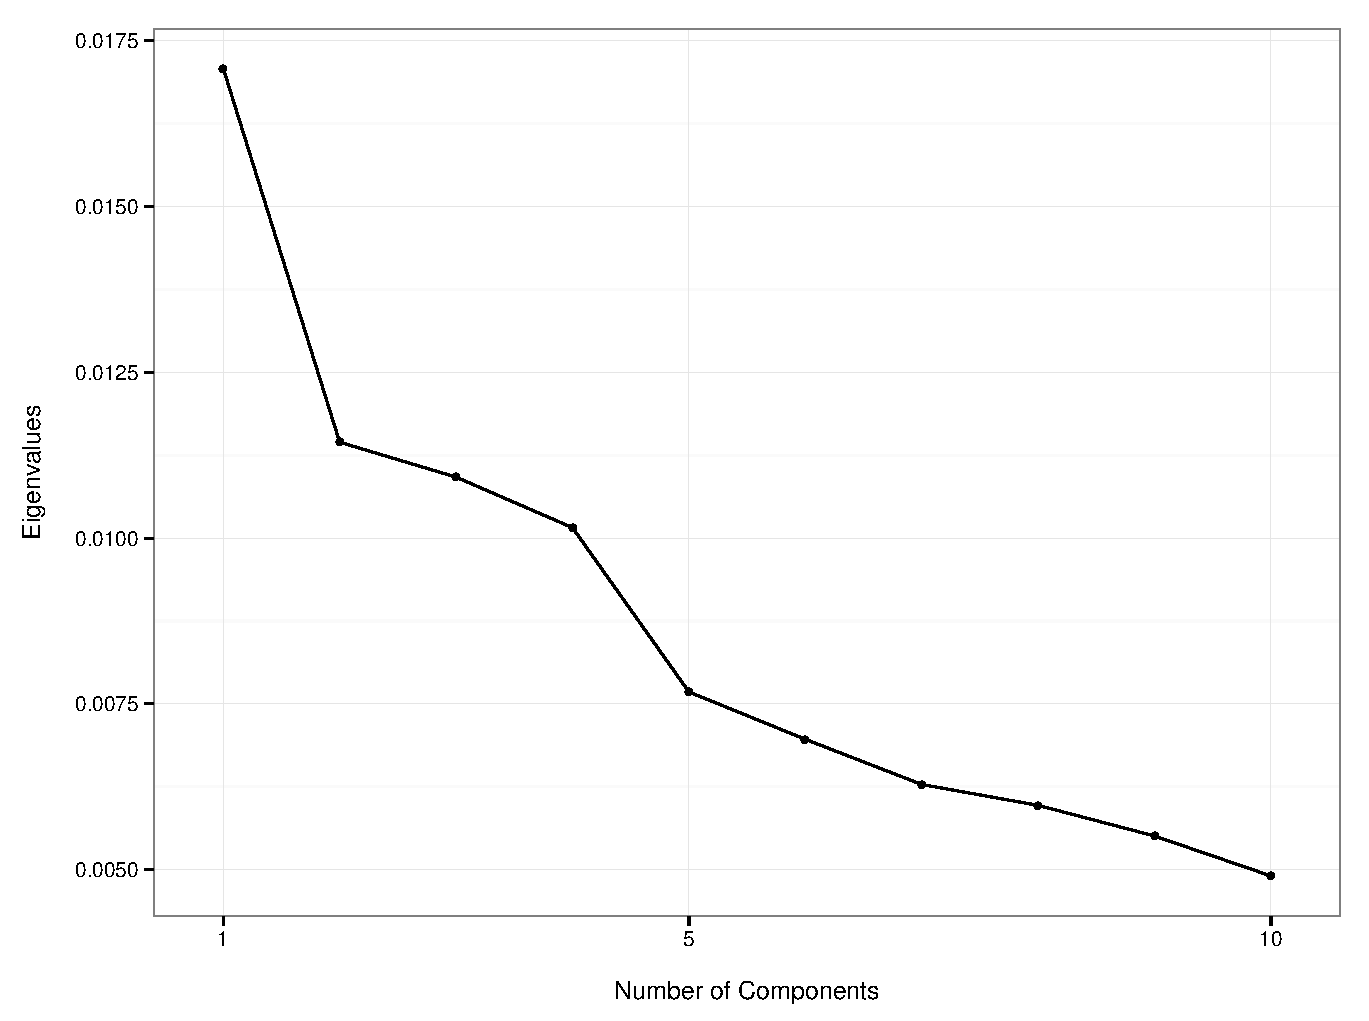
\includegraphics[scale=0.5]{figures/scree_plot.pdf}
    \end{center}
\end{figure}

\subsection{Data Access and Replication}

The FinStress Index set can be found at:
\url{https://github.com/christophergandrud/EIUCrisesMeasure}. This website also includes the complete replication material for creating FinStress.

\section{Validation and Description}\label{results}

The solid lines in figures \ref{compare_1} and \ref{compare_2} show FinStress for a wide selection of countries. What does this dimension actually represent? Grimmer and Stewart \citeyearpar[267]{Grimmer2013} argue that to validated the results of a text analysis we need ``careful thought and close reading \ldots extensive and problem-specific validation''. As such, we took a number of approaches to answer this complex question. We used a variety of  techniques to examine how the texts relate to the estimated scores. Following \cite{Spirling2012} we used a random forests ``regression'' \citep{Breiman2001,jones2015}, as well as stem-component correlations to examine the relationships between word stems from the texts and FinStress. We also qualitatively examined a selection of the tests classified as being at various FinStress levels. Second, we extensively compared the Index to other measures of financial market stress and crisis using a variety of statistical and qualitative techniques.

\subsection{Random forests and correlations}\label{random-forests}

Spirling \citeyearpar[88-90]{Spirling2012} demonstrated the usefulness of using random forests regressions to explore what principal components from textual analyses represent. To use this tool to explore our data, we first created a document-term frequency matrix from the stemmed documents. Effectively this is a \(k \times s\) matrix recording the frequency of each stem in \(\bm{S}\) for each document in \(\bm{K}\). \emph{The document-term matrix clearly does not preserve word order, so should only be thought of as one of a number of ways of assessing validity}. We removed sparse terms, i.e.~kept only stems that were found in 90 percent of the documents. Random forests regressions, as opposed to ordinary least squares regressions, are useful for exploring this data's associations with the estimated principal components because it can handle many variables--in this case 1,116 stems--relative to the number of documents--12,377.

We focus on estimated variable importance. Variable importance in this context functions as a measure of how well the frequency of a given stem in a text allows the model to predict the FinStress score for that text.\footnote{Specifically, importance is measured in terms of the percentage increase in mean squared error (MSE) after permuting the variable. If a variable is important, then permuting it will decrease predictive performance, i.e. increase MSE. We conducted the random forests regressions using the \texttt{rfsrc} function from the \textbf{randomForestSRC} R package \citep{randomForestSRCCite}.} Key results are shown in Figure \ref{rf_importance}.

Unsurprisingly, a number of the stems with the largest variable importance are ``bank'', ``financi'', and ``loan''. Terms with these stems were used to select the texts. The prevalence of these terms and others that are clearly related to the financial sector, such as ``interest'', ``rate'', and ``fund'', indicate that FinStress is indeed about financial sector conditions and not some other topic. Words relating to the direction of financial conditions are important including, ``growth'' and ``rise''. We can see that words relating to the the macro-political economic environment of finance are also important, including ``govern'', ``imf'', and ``currentaccount''.

Table \ref{stem_correlations} shows a selection of correlations to provide a sense of the general directions of the relationships between the stems and the Index not provided by the random forest variable importance estimates. We can see that a number of terms related to debt, financial assistance, the International Monetary Fund, and aid are positively related to FinStress. This suggests that the positive direction of the scale is in fact capturing periods where policymakers perceive higher financial market stress. Words that are generally about positive credit conditions, such as ``growth'', ``surplus'', and ``boom'' are negatively associated with the Index. This suggests that the lower end of the scale indeed indicates more positive financial market conditions. Finally, we can see that adjectives that have seemingly opposite meanings--``stronger'' and ``weaker''--are both negatively associated with the Index. Such a finding indicates that a KPCA approach is useful compared to context-less bag-of-words approaches.

\begin{figure}
    \caption{40 Stems Estimated to be the Most Important for Predicting EIU Perception of Financial Market Stress Index}
    \label{rf_importance}

    \begin{center}
        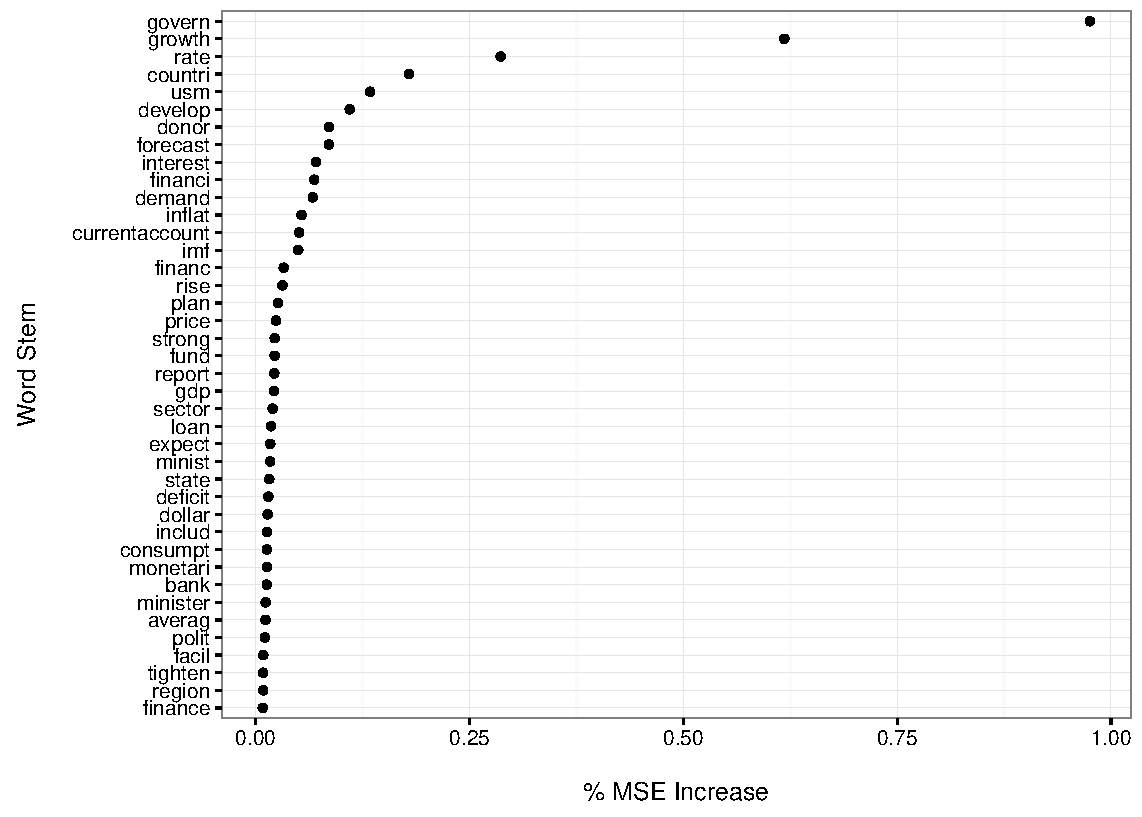
\includegraphics[scale=0.5]{figures/rf_stem_importance.pdf}
    \end{center}

\end{figure}

% latex table generated in R 3.2.1 by xtable 1.7-4 package
% Mon Jun 29 14:16:00 2015
\begin{table}[ht]
\centering
\caption{Selection of Word Stems and Correlations with EPFMS Index} 
\label{stem_correlations}
\begin{tabular}{lr}
  \hline
Stems & Correlations \\ 
  \hline
imf & 0.34 \\ 
  assist & 0.34 \\ 
  aid & 0.28 \\ 
  debt & 0.24 \\ 
  paid & 0.19 \\ 
  strain & 0.09 \\ 
  boom & -0.14 \\ 
  surplus & -0.14 \\ 
  rise & -0.14 \\ 
  weaker & -0.16 \\ 
  stronger & -0.17 \\ 
  growth & -0.28 \\ 
   \hline
\end{tabular}
\end{table}


\begin{table}
    \caption{Portions of Texts EIU Reports with Country-\textbf{Maximum} FinStress values (selected countries)}
    \label{text_selections_max}
    	\begin{center}
        \begin{tabular}{c c c | m{10cm}}
            \hline
            Country & Month-Year & FinStress & Text Selection \\
            \hline\hline
            Brazil & August 2003 & 0.58 & While domestic lending to industry picked up in the second half of the year, consumer credit has been flat \ldots the effects of exchange rate depreciation on input costs in 2002 is still being felt in continued pressure on consumer prices in early 2003, requiring stringent monetary policy to suppress inflation. \\[0.5cm]

            Latvia & June 2009 & 0.65 & The economy is slowing sharply, and real GDP contracted by 18\% in the first quarter of 2009 \ldots In the current economic climate most Latvian households and companies will concentrate on reducing their debts; foreign banks operating in Latvia are also trying to reduce their exposure to Latvia by lending less. \\[0.5cm]

            Ireland & April 2011 & 0.78 & Irish households are highly indebted. Private consumption will therefore be constrained as households rebalance their balance sheets and as credit conditions remain tight in 2011-13. Investment will continue to shrink in 2012 as the collapse of the construction industry maintains momentum \ldots [the] most recent stress tests reveal the complete failure of earlier attempts to assess the impairment of the banks' balance sheets. Of particular note is the fact that no serious provision had previously been made for losses on the banks' mortgage lending, despite a massive collapse in the residential property market that has been ongoing for some years. \\[0.5cm]


            \hline
    \end{tabular}
    \end{center}
\end{table}


\begin{table}
    \caption{Portions of Texts EIU Reports with Country-\textbf{Minimum} FinStress Values (selected countries)}
    \label{text_selections_min}
    	\begin{center}
        \begin{tabular}{c c c | m{10cm}}
            \hline
            Country & Month-Year & FinStress & Text Selection \\
            \hline\hline
            Brazil & August 2005 & 0.05 & By continuing to meet the target for the primary fiscal surplus despite strong political pressure to increase spending on social programmes, and by increasing the benchmark Selic overnight rate until inflation began to subside in June, the government has confirmed its cautious stance. Apart from keeping a rein on inflation, this has helped to maintain confidence in the financial markets. \\[0.5cm]

            Latvia & March 2006 & 0.18 & The BoL [Bank of Latvia] has tried to curb the current lending boom by raising the mandatory reserve requirements for banks from 4\% to 8\% in 2005, in two steps. Further increases seem unlikely, as Latvian customers could be served from other EU countries if the costs of banking in Latvia become excessive. \\[0.5cm]

            Ireland & January 2007 & 0.06 & Private consumption will be fuelled in 2007 by strong employment growth, solid real wage increases, tax cuts, lower inflation and the maturing of a generous government-financed savings scheme \ldots Strong business confidence and a still-booming construction sector will bolster growth, but an anticipated cooling of the housing market will account for the deceleration over the outlook period. \\[0.5cm]


            \hline
    \end{tabular}
    \end{center}
\end{table}


\subsection{Qualitatively examining texts}

While random forest regressions and correlations allow us to summarize more than 12,000 documents, they only allow us to examine how individual words are related to the FinStress estimates. This is explicitly not how FinStress is estimated. As such, we also looked at a selection of full texts to get a more complete picture of what types of documents were classified as having high and low FinStress scores.

Tables \ref{text_selections_max} and \ref{text_selections_min} provide snippets of texts with country maximum and minimum FinStress scores. We selected the countries such that we have a range of maximum scores. Brazil had a relatively low maximum FinStress score in the sample--0.58 in 2003. The text this score is from reflects this relatively middling score. It highlights that lending to industry has increased, while ``consumer credit has been flat'' and consumer prices are increasing. Latvia had a higher maximum FinStress score--0.65 in 2009--and the text this score is generated from clearly describes a more troubled financial sector. The economy is noted to be ``slowing sharply'' leading households and companies to focus on reducing debts, and foreign banks reducing their exposure to the country. Ireland had a relatively high maximum FinStress score--0.78 in 2011. The text this score is estimated from describes a highly troubled banking system that is going through a painful restructuring process  is reducing the supply of credit to the economy.

The texts that created country-minimum FinStress scores--shown in Table \ref{text_selections_min}--describe ``confidence in financial markets'' in Brazil (2005), a ``lending boom'' in Latvia (2006), and ``strong business confidence'' in Ireland (2007). Importantly, in the Latvian and Irish cases the texts are not without clear concerns that the boom may not continue into the future. So while low FinStress scores appear to be reflecting financial markets with strong credit provision embedded in these texts is a concern that the boom may be peaking. This is an important finding to keep in mind when interpreting the substantive meaning of low FinStress scores. It is an issue that \cite{gandrud_pepinsky2015} formally model in separate work and are able to empirically test using FinStress.

\subsection{Compared to other crisis
measures}\label{comparison-to-other-crisis-measures}

How does FinStress compare to previous ways of measuring and timing financial market stress and crisis? We first compare the Index to the dichotomous measures of banking crisis developed by \cite{Reinhart2009} and \cite{laeven2013}, as well as Romer and Romer's \citeyearpar{Romer2015} continuous measure.

We anticipate that the Reinhart and Rogoff and Laeven and Valencia measures should be positively correlated with FinStress, they are both sensitive to extreme stress, particularly if there is a large government response. At the same time, because of the other issues we find present in these variables, the correlation should be fairly weak. More important than the--not particularly informative--simple correlation between FinStress and the rare events binary variables is that we expect the binary measures to miss the build-up to crises, cases where there is a build-up in pressure but the full-blown crisis does not develop, and poorly time decreases in extreme stress. Using data transformed in the way discussed below, FinStress and Laeven and Valencia's banking crisis measure do have a positive correlation coefficient as expected and, as expected, it is weak at 0.088. Similarly, FinStress and Reinhart and Rogoff's measure have a correlation coefficient of 0.087. Romer and Romer's more similar continuous and contemporaneously text-based index is more strongly correlated with FinStress at 0.248. Note that all correlations are statistically significant at the 5\% level.\footnote{We use Table 1 in \cite{Romer2015} to recreate their data set. The Laeven and Valencia's data is from: \url{https://www.imf.org/external/pubs/cat/longres.aspx?sk=26015.0}.
  Accessed May 2015. Reinhart and Rogoff's data was downloaded from:
  \url{http://www.carmenreinhart.com/data/browse-by-topic/topics/7/}.
  Accessed May 2015.}

%The third issue concerns errors because they use human coding. Not sure how easy it is to find here, but maybe there are idiosyncrasies in their dataset we pick up with a more automated approach.

To follow up on the expectation that our measure is capturing the same concept, but with more nuance, especially in magnitude and over time, figures \ref{compare_1} and \ref{compare_2} plot the four measures for a wide selection of countries.\footnote{There are some limitations in comparability due to the different periods of coverage of the different indices. \cite{Romer2015} in particular largely do not include the most recent crisis in their sample as they did not collect data past 2007. We also had to make a number of transformations and assumptions to be able to  compare directly the different data sets. First, the Laeven and Valencia and Reinhart and Rogoff data are recorded at yearly intervals. We assume that the crisis start and end dates they referred to were in the middle of the year, i.e. June.\footnote{In the period covered in figures \ref{compare_1} and \ref{compare_2} this improves their fit with events, as many of the 2008 crises became especially apparent after Lehman Brothers collapse in September 2008.} Second, we rescale Romer and Romer's 16-point scale (in effect 14-points because they do not classify any country-quarter in their sample as being at the upper two positions on their scale) to be between 0 and 1 using the same method as discussed above for FinStress. Finally, it should be noted that \cite{Romer2015} only cover a selection of OECD countries and \cite{Reinhart2009} only cover 70 countries and their data has been updated least recently.} The solid lines in figures \ref{compare_1} and \ref{compare_2} show the FinStress Index. The dashed lines show Romer and Romer's (rescaled) measure. The shaded boxes show the periods where \cite{laeven2013} and \cite{Reinhart2009} classify the existence of a banking crisis. \cite{laeven2013} identify eight ``borderline'' crises in this period, in that the countries almost meet their systemic banking crisis definition because they only used two rather than three policy responses.\footnote{The cases are: France, Hungary, Italy, Portugal, Russia, Slovenia, Sweden, and Switzerland.} Some of these borderline cases are shown in the figures \ref{compare_1} and \ref{compare_2}.

In many cases--conditional on the coverage of each data series--the indices do substantively overlap. Comparisons with \cite{Romer2015} are limited, but we can see that, where comparable time series are available, there are cases where FinStress and their index are similar: for example, both indices increase in the US from early 2007. A notable difference is how Romer and Romer classify Japan as being without stress from mid-2005, while FinStress remains relatively high, especially compared to many other economically developed countries at that time. While both indices classify Iceland as being under stress in the late 2000s, the timing is different. Romer and Romer classify Iceland as in stress\footnote{They classify Iceland as being in a ``minor crisis'' in the second half of 2006 and a ``credit  disruption'' in the first half of 2007.} in 2006-2007. This is earlier than not only a marked increase in the FinStress Index, but also Reinhart and Rogoff and Laeven and Valencia's timing.

\cite{Reinhart2009} sometimes date the start of a crisis before \cite{laeven2013}--notable cases include Iceland and Ireland. This could reflect the slightly different definitions that they use. As summarized in the Appendix's Table \ref{comp_table}, \cite{Reinhart2009} date crises from when bank runs occur. \cite{laeven2013} begin the crisis clock when there is not only significant financial system distress, but also when the government follows the distress with a policy response.

We would like to point out that these findings have theoretical relevance. We indicate that high levels of stress should appear where there is crisis in the dichotomous codes, but the reverse may not be true--the dichotomous indices may miss a building crisis as perceived at the time. This means that Laeven and Valencia and Reinhart and Rogoff should have more Type II errors--there are signs of a crisis but they miss them. The Laeven and Valencia coding is stricter in that countries have to both experience distress and have a particular policy response to it, so the associated FinStress levels should be higher. Finding evidence supporting these expectations would reinforce our arguments about the problems with their measures and FinStress' validity for what we want to capture.

We do find that the mean FinStress level during periods that Laeven and Valencia classify as crises--i.e., financial market stress reached the point where politicians responded using a pre-specified set of policies--is higher than non-crisis periods.\footnote{0.55 and 0.51, respectively. This is a statistically significant difference using one-sided and two-sided t-tests.} Though developing countries tend to have higher FinStress scores, countries defined by Laeven and Valencia as in crisis in both groups have FinStress scores around 0.55 on average. Those not in Laeven and Valencia crises have lower scores. Please see the Online Appendix for a discussion of the distributions of FinStress scores in developed and developing economies. Overall, developing countries have more stressed financial markets, which does not always lead the government to take policy measures that Laeven and Valencia are looking for. The fact that the mean FinStress is higher during periods that Laeven and Valencia classify as crises, but not dramatically, supports the proposition that they miss considerable periods of budding and high stress and perhaps suffer from more Type II errors.

We can use FinStress to follow the progression of crisis intensity over time. Laeven and Valencia \citeyearpar[227]{laeven2013} comment that part of the problem with dating financial crises is that each develops differently:

\begin{quote}
    Some crises evolve gradually, gaining speed as the ripple effects from a seemingly small shock propagate forward in time \ldots other episodes happen more abruptly and are often the result of sudden stops.
\end{quote}

\noindent FinStress' real-time continuous measurement and monthly periodicity allows us to distinguish these types of crises. This has relevance when thinking about how crises develop over time. For example, we can see in Figure \ref{compare_2} that financial market difficulties in the United States built over a long period of time, with a few spikes during notable banking difficulties, e.g. Lehman Brothers' collapse. Conversely, countries such as Germany, Hungary, and Iceland clearly have much more sudden periods of perceived financial distress. The Greek case presents an interesting additional trajectory. There is a notable spike in Greek financial stress in 2008--when both \cite{Reinhart2009} and \cite{laeven2013} determine a crisis had started. This is then followed by a stable period, followed by a sudden uptick in 2010, which was when a possible government default severely threatened the banking system.

Kazakhstan is notable for another trajectory: a very rapid stress onset and just as rapid dissipation (see Figure \ref{compare_2}). In late 2009 there was a prominent spike in perceptions of financial market stress directly related to a credit crunch that hit the country's banking sector as an after shock of the Global Financial Crisis. According to an IMF assessment,\footnote{See: \url{http://www.imf.org/external/pubs/ft/survey/so/2010/car081710a.htm}. Accessed November 2015} a large and quick policy response--facilitated by the sizable National Oil Fund--within a few months returned stability to the country's banking system. Kazakstan's FinStress score reflects this by returning to almost its previous trend level at that time.

FinStress allows us to explore why different crises follow different trajectories over a series of months. An annual binary definition of crises does not allow us to capture these changes.

We can use FinStress to identify periods where financial market conditions were perceived to be worsening, though for whatever reason these perceptions changed before other measures would record a financial crisis. Australia, Brazil, and the Czech Republic, among others, in late-2008/2009 are notable examples. They all have clear spikes in perceptions of stress shortly after Lehman Brothers collapsed in the US. Fairly quickly thereafter, their FinStress scores returned to previous levels. Laeven and Valencia and Reinhart and Rogoff do not distinguish these periods from those with little financial market stress. While there were not widespread bank failures in these cases, the fact that they are treated as the same as placid periods by the binary measures makes it impossible to study how policy choices may have contributed to heading off worse stress.

The advantages of FinStress are also apparent for timing the end of heightened financial market distress. This is a particularly difficult issue for the established binary indicators. Crisis onset is typically well defined by these measures, but they rarely have a clear or non-\emph{ad hoc} way of determining when a crisis has ended. Though we are limited by the time period coverage of the EIU texts we have at our disposal, it is clear that some countries, notably the Netherlands, Switzerland, the United Kingdom, and the United States, were perceived to be having improved financial market conditions from about 2010. Other countries, particularly Eurozone countries in Western and Southern Europe plateaued at a high level through the end of 2011, a period that corresponds with the Eurozone crisis. Laeven and Valencia's measure uses an \emph{ad hoc} definition of crisis termination (see above) and so simply classifies these entire periods as crises with equal intensity. Not only does FinStress allow us to more accurately date when conditions were seen to have improved, but it also allows us to study the trajectory of these improvements.

Overall, the similarities between FinStress scores and other measures of crises suggest that the Index does capture financial market stress in that higher FinStress values are indicative of higher levels of perceived financial market stress. At the same time, the differences between the measures indicate that FinStress sheds unique light on processes not captured well by previous indices.

\begin{figure}
    \caption{Comparing Perceptions of Financial Market Conditions to \cite{laeven2013} and \cite{Reinhart2009} (1)}
    \label{compare_1}
    \begin{center}
        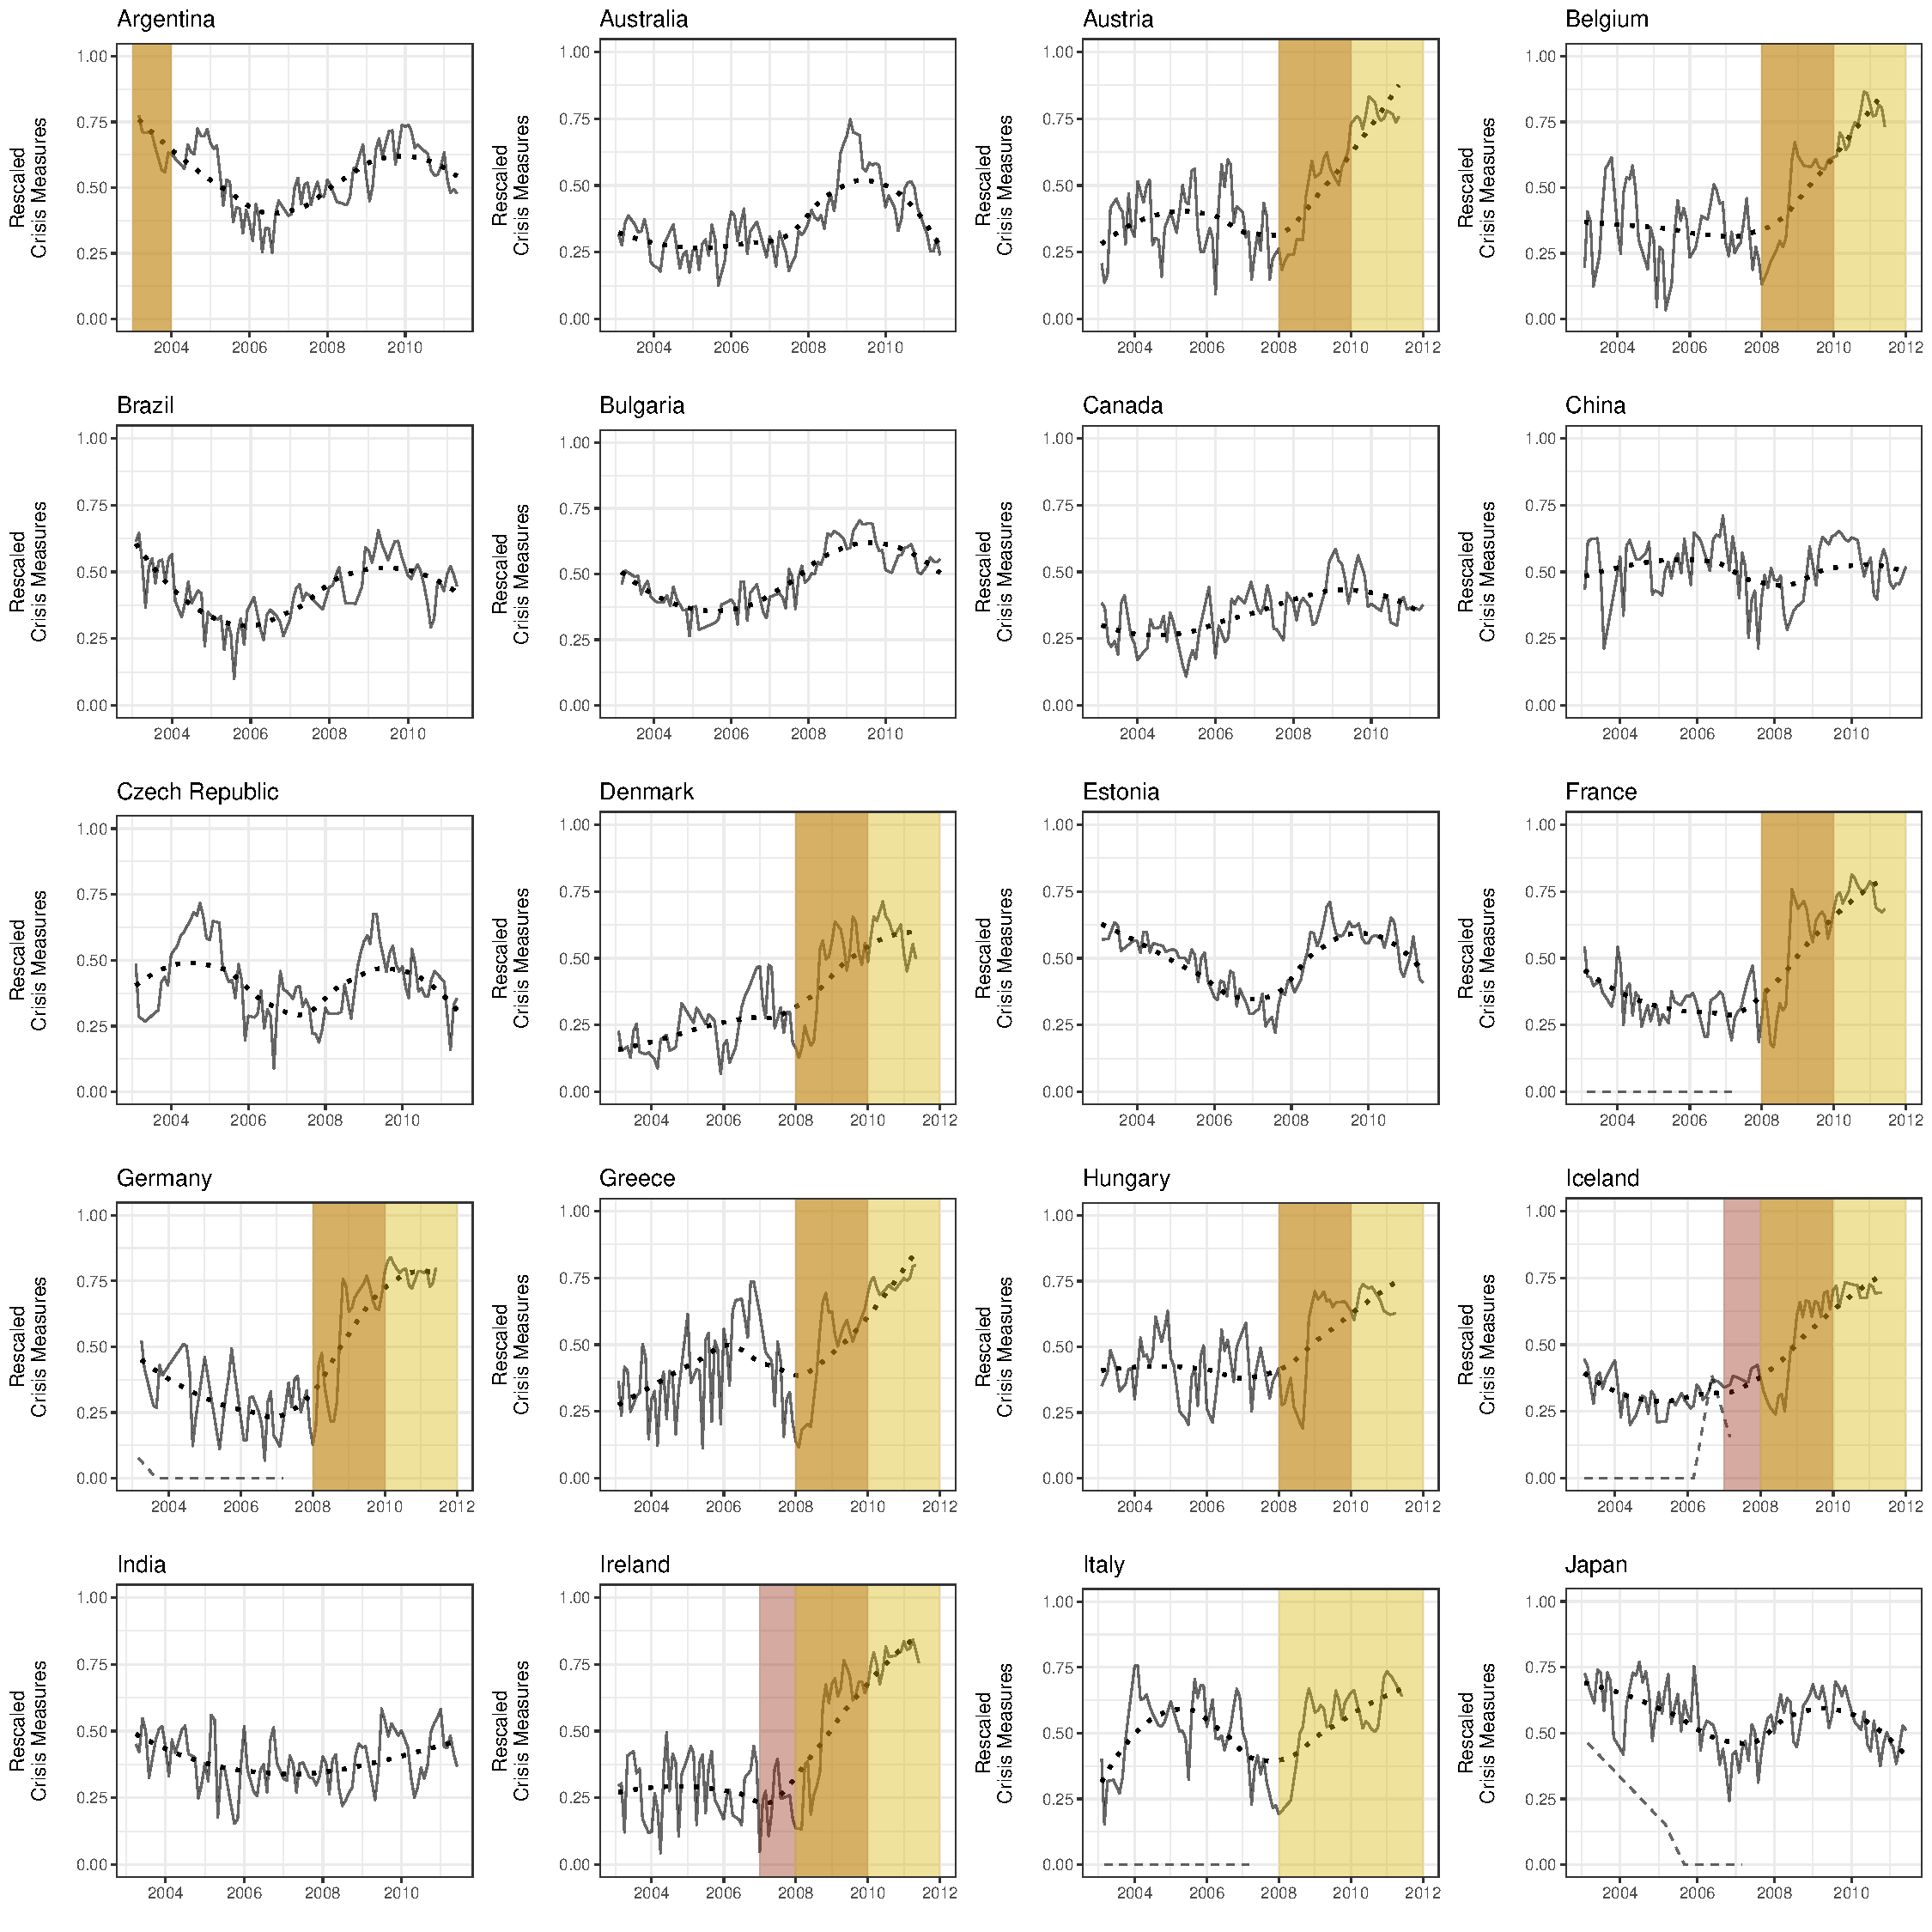
\includegraphics[scale=0.4]{figures/compare_to_lv_rr.pdf}
    \end{center}

    {\tiny{Solid lines show the FinStress Index. Dotted lines represent a loess smoother of these series. \\

    Yellow shaded areas indicate periods that \cite{laeven2013} classify as systemic banking crises. Note that crises are automatically terminated at the end of 2011 due to the series not extending beyond this point, not necessarily because the crisis finished. \\

    Red shaded areas indicate periods that \cite{Reinhart2009} classify as banking crises. Note that crises are automatically terminated at the end of 2009 due to the series not extending beyond this point, not necessarily because the crisis finished. \\

    Orange areas indicate periods where a crisis is recorded for both measures.}}
\end{figure}

\begin{figure}
    \caption{Comparing Perceptions of Financial Market Conditions to \cite{laeven2013} and \cite{Reinhart2009} (2)}
    \label{compare_2}
    \begin{center}
        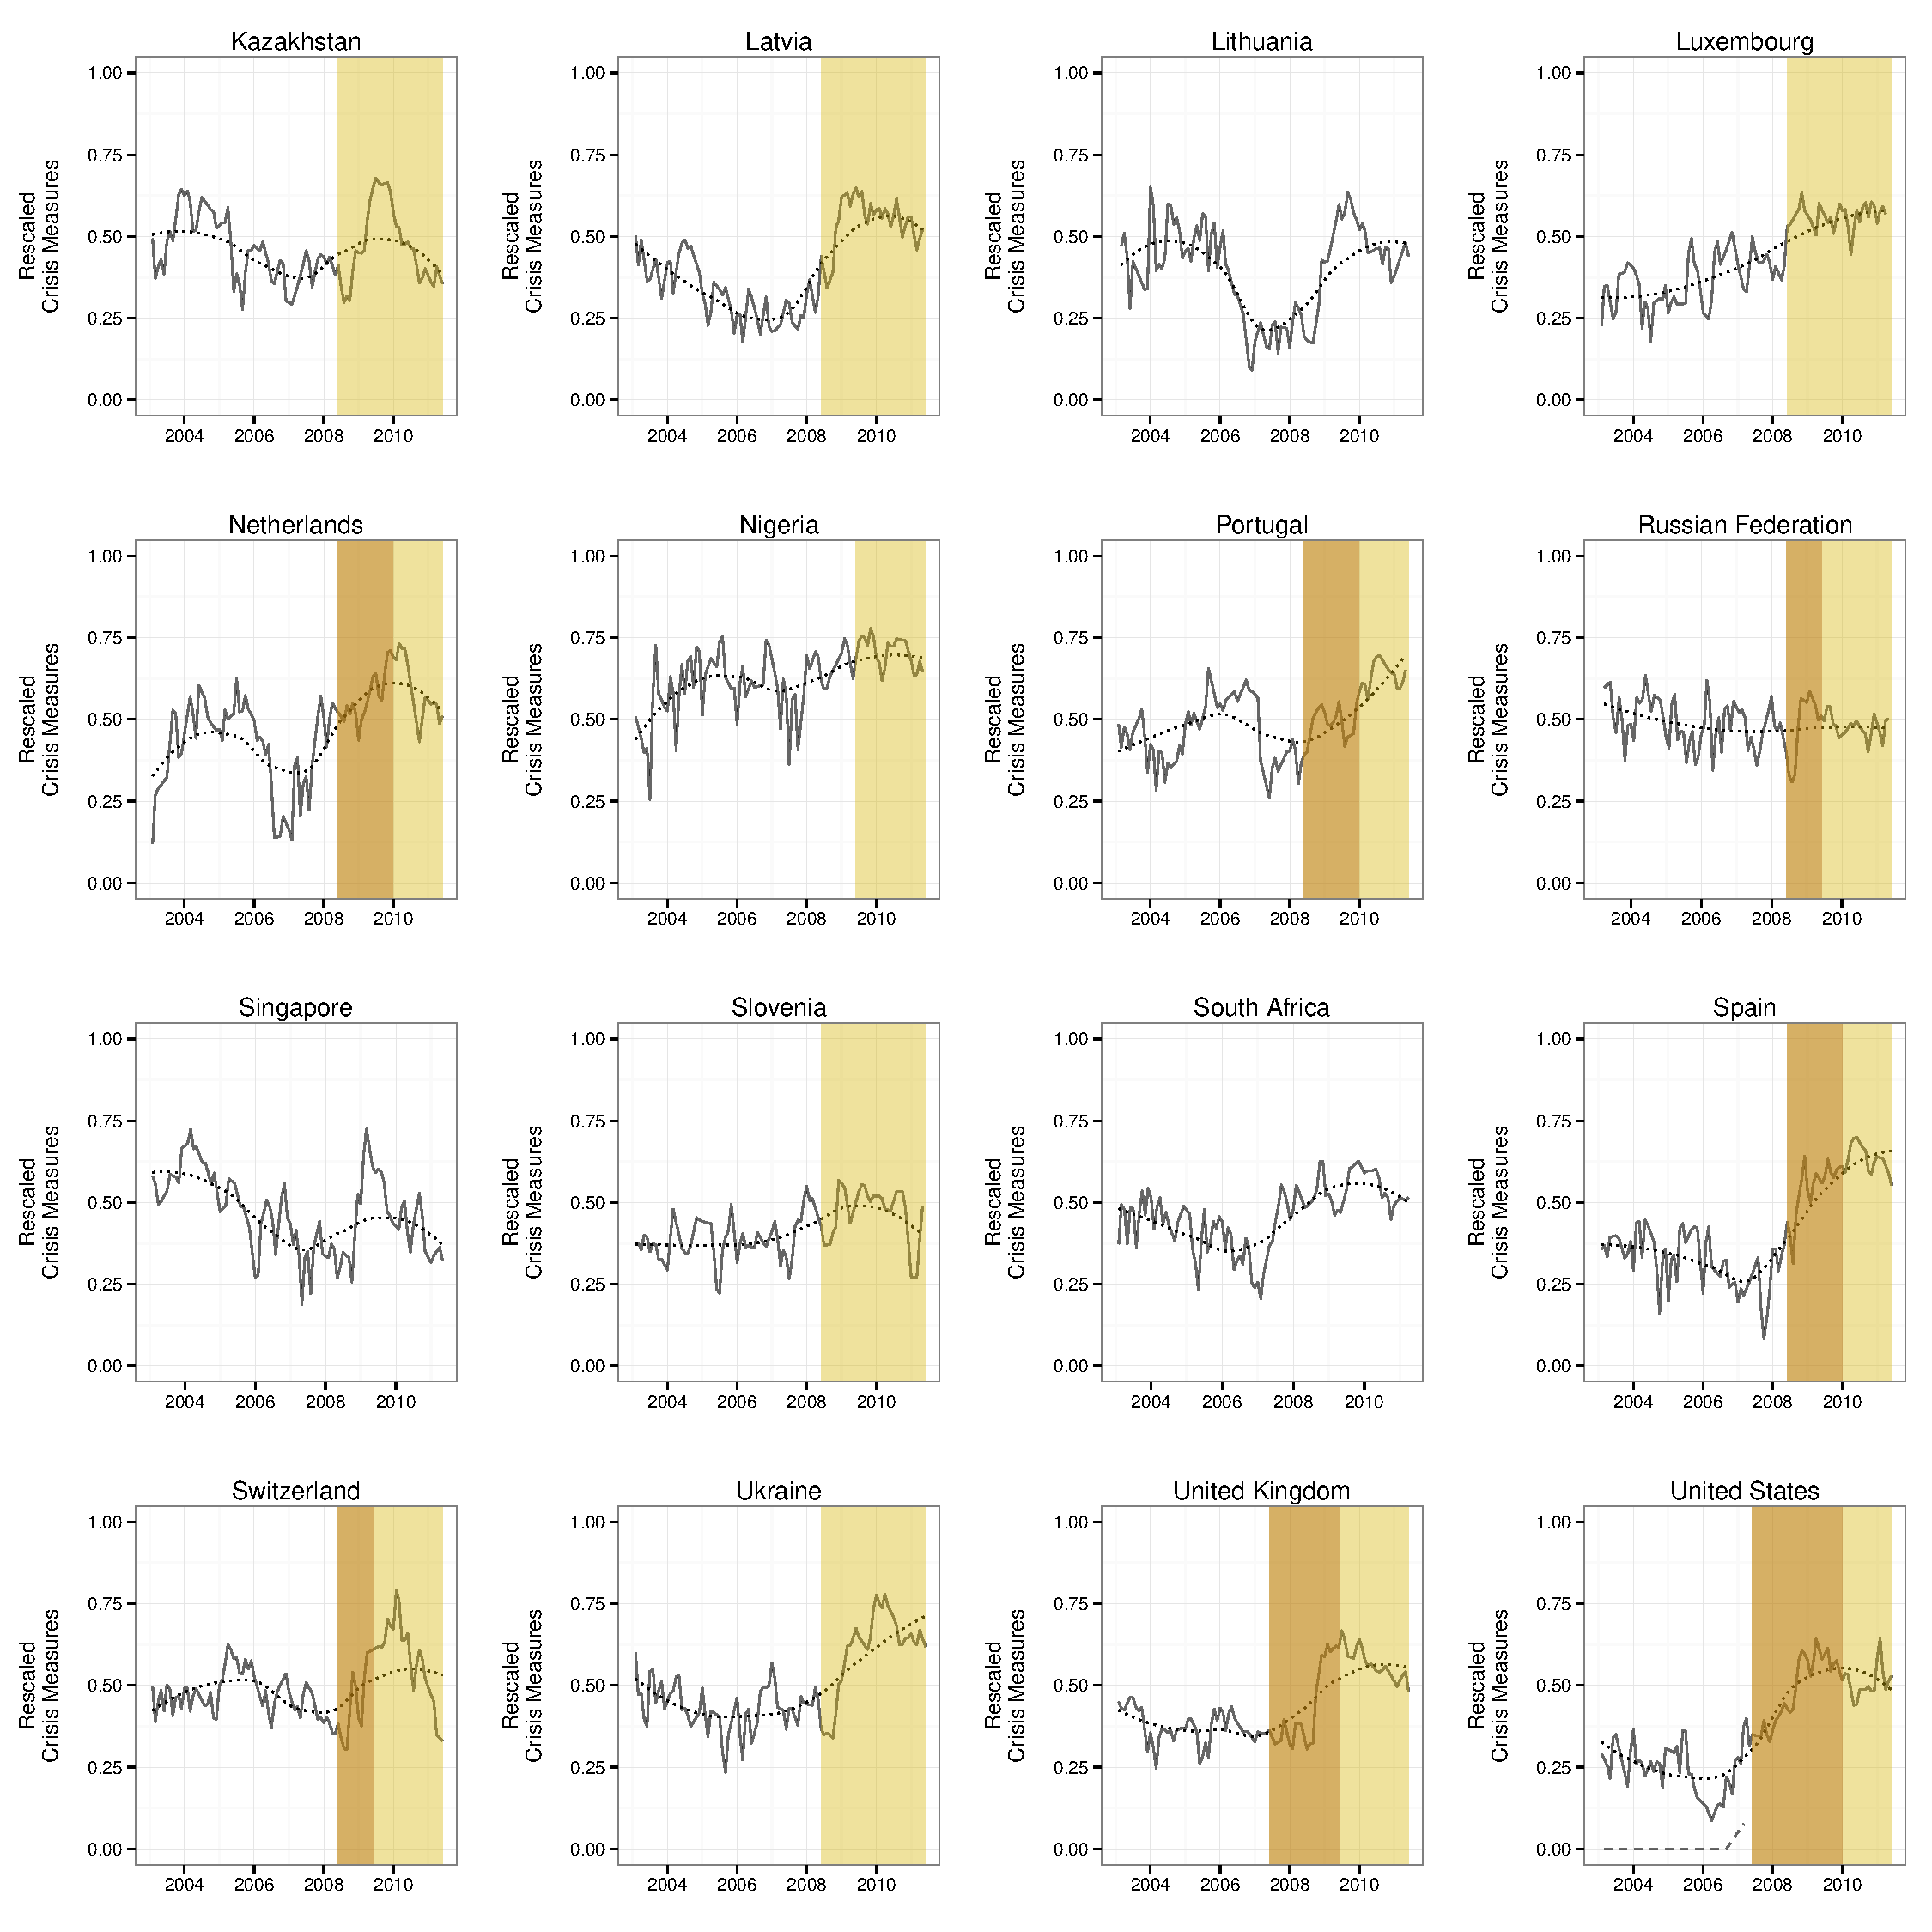
\includegraphics[scale=0.4]{figures/compare_to_lv_rr_2.pdf}
    \end{center}

    {\tiny{See Figure \ref{compare_1} for notes.}}
\end{figure}

\begin{figure}
	\caption{Comparing Annual Mean Perceptions of Financial Market Conditions with Components of the CAMELS System from \cite{Andrianova2015}}
    \label{camel_plot}
    \begin{center}
		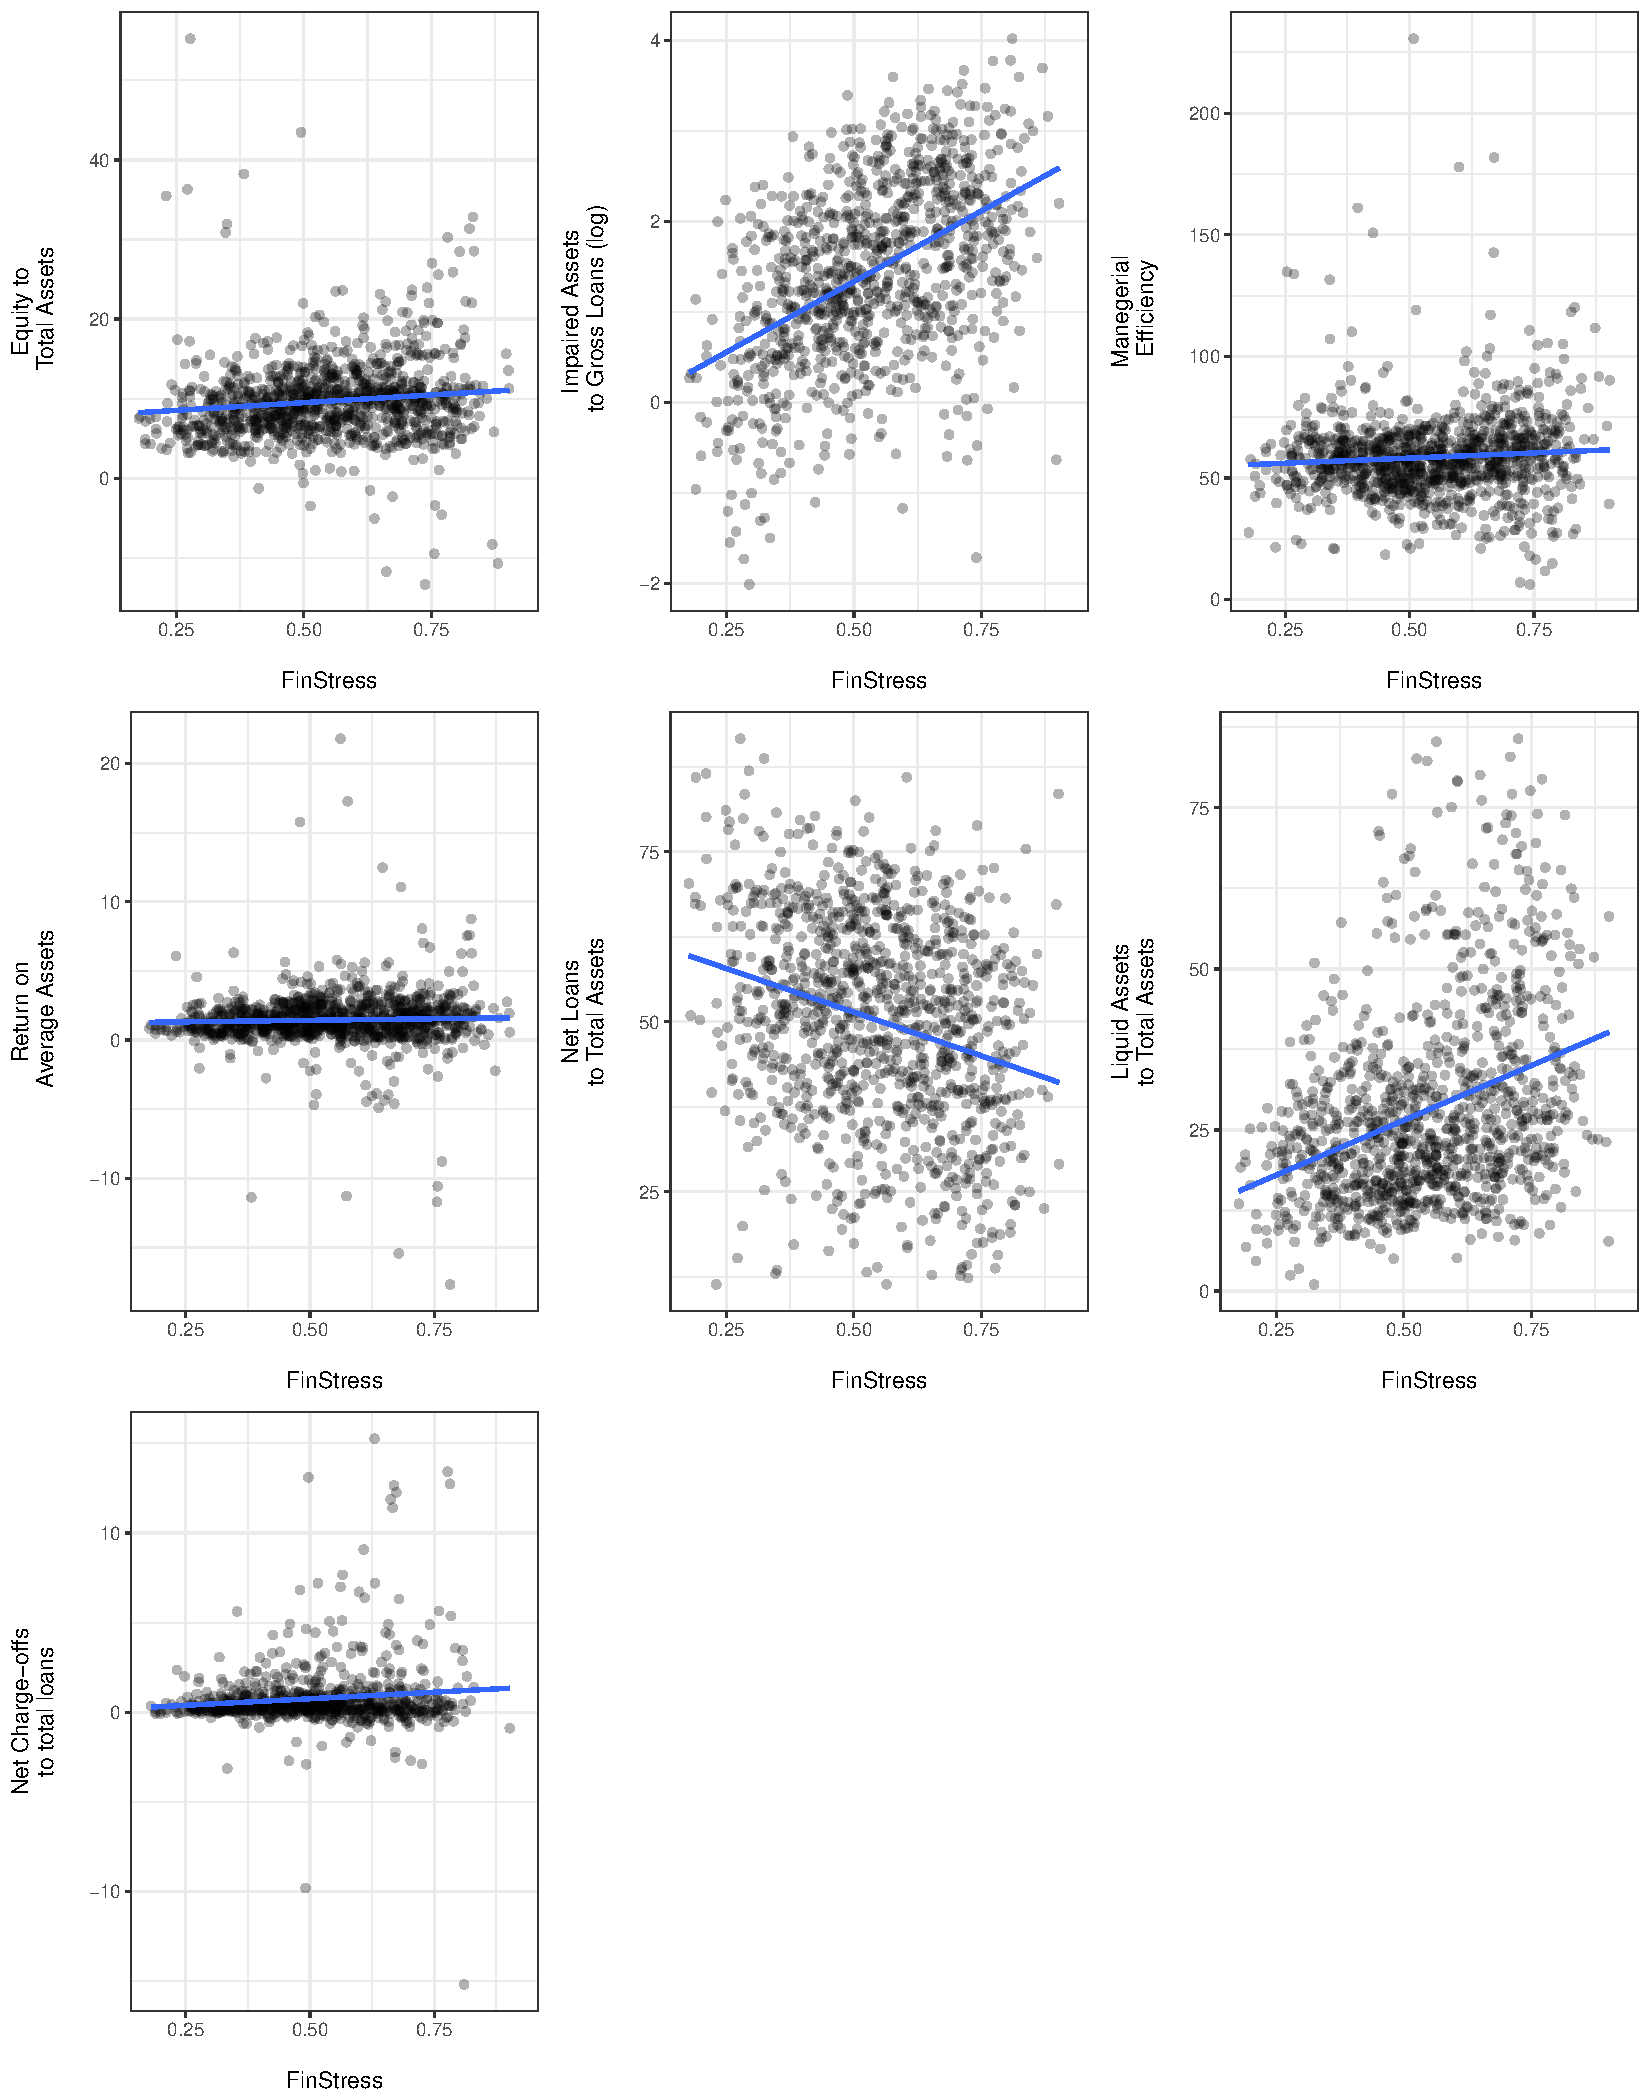
\includegraphics[scale=0.55]{figures/fin_fragility_compare.pdf}
	\end{center}
\end{figure}

\subsection{Comparison to accounting measures of banking system fragility}

\paragraph{CAMELS}

How does FinStress compare to the components of the CAMELS system of bank soundness? We used annual FinStress means to compare it to annual national aggregates of the CAMELS variables in \cite{Andrianova2015}. Figure \ref{camel_plot} shows the bi-variate relationships between FinStress and these variables. FinStress is statistically significantly associated with six of the seven CAMELS variables at the 5\% level.\footnote{It is not significantly associated with Return on Average Assets. Please see the correlation table in the Appendix for details.} FinStress is strongly associated with three of the CAMELS variables in that there is a correlation coefficient greater than 0.25 or less than -0.25. These variables are impaired assets to gross loans, net loans to total loans, and liquid assets to total assets. See Figure \ref{cor_camel} in the Online Appendix for the full correlation matrix.

FinStress is strongly positively associated with impaired assets.\footnote{The log of impaired assets--it is a highly skewed variable--is associated with FinStress with a correlation coefficient of 0.43, significant at all standard levels} Impaired assets are otherwise often known as non-performing loans. Banks are solvent when their assets (e.g. loans and the income they generate) can cover their liabilities (e.g. deposit withdrawals). Impaired assets greatly threaten banks' ability to meet their obligations and so threaten their solvency. As such, it seems as though FinStress is closely related to bank balance sheet health.\footnote{Note the outliers in the middle-top panel of Figure \ref{camel_plot} that seemingly have both high stress and very low impaired loan levels. The countries with (log) impaired loans less than 0 and FinStress greater than 0.6 are: the Democratic Republic of Congo (2008, 2010), Cote d'Ivoire (2011), Estonia (2004), Guinea-Bissau (2011), Kyrgyzstan (2007, 2011), Seychelles (2006, 2007), Sudan (2008), and Uzbekistan (2004). These countries also have considerable missingness in their Bankscope data in that many banks in these countries do not report data. It is likely that either the low impaired loan scores are based on reporting by only less troubled banks or there is inaccurate reporting. In these cases it is likely that FinStress is a better measure of banking system health.}

Initially, it may seem strange that FinStress is positively associated with liquid (e.g. cash) asset ratios. Banks with more liquid assets are less likely to become insolvent because they can use these assets to meet their liabilities. However, high liquid asset ratios can be a manifestation of a stressed financial system as banks create large liquid asset stockpiles when they are reluctant to lend--take on less liquid assets. This behaviour restricts credit to the wider financial system and economy. Following the Lehman Brothers collapse in 2008 an extreme version of this occurred, becoming known as a ``credit crunch''. \cite{Andrianova2014} find that African banks have very high liquid asset ratios because lending risks are high, so banks are reluctant to make new loans. To a large extent net loans and liquid assets are inversely related. As such we find a negative relationship between net loans and FinStress--banks in countries with higher FinStress scores are making fewer loans and instead are hording liquid assets.

\paragraph{Global random forest regression}

To conduct a global assessment of how the various quantitative measures of bank and banking system stress relate to FinStress we conducted a random forest regression. We include in the regression CAMELS indicators and a number of other indicators from the Global Financial Development Database that the World Bank classified as being related to banking system stability \citep{worldbank2015} including Z-Scores.\footnote{Variables from the GFDD include: provisions to NPLs, stock price volatility, regulatory capital to assets, capital to assets, credit to deposits, stock market returns, and private sector credit provided by banks and other financial institutions. The last two are not classified by the GFDD as banking ``stability'' indicators, but we included them as they may be substantively important.} Our main reason for using random forest regressions is that we are examining the relationships between many highly correlated variables and FinStress. As all of the right-hand side variables are country-year aggregates, we examine their relationship with country-year mean FinStress levels.

It should be noted that the random forest regressions are based on a slim sub-sample for which we have FinStress scores. There are 1,678 country-years for which we have average FinStress scores, but due to missingness issues discussed above, only 394 of these have complete information across the included indicators and thus are included in the random forest regression.

With that significant caveat noted, Figure \ref{rf_var_importance} shows the importance each variable plays on average for predicting FinStress levels. We can see that, impaired loans are found to be the most important variable for predicting FinStress levels in this sub-sample.\footnote{In a sample of all countries, exchange rate change is also relatively important, though when the sample is subsetted to look only at high income countries, it has no impact on reducing predictive error. This makes substantive sense as in the period under examination exchange rates in high income countries were relatively stable, even during crises. Stress in developing countries is closely related to foreign exchange disruptions and the currency asset-liability mismatches banks face in these situations.} The second most important is highly related to impaired assets--return on average assets. When there are more non-performing loans the average return on all loans is lower. The third most important variable, again similar to impaired loans, is bank provisioning relative to their non-performing loans. Z-Scores are a fairly poor predictor of FinStress. Please see the Online Appendix for a detailed exploration of the relationship between FinStress and Z-Scores. The main conclusion of this work is that Z-Scores, at least as measured by the World Bank are a sub-optimal measure for examining how banking stress changes over time and should be avoided in research that requires a measure of this.

Figure \ref{rf_partial_depend} shows the predicted values from repeated draws of FinStress averaged within the values of the other variables included in the random forest regressions \citep[see][14]{jones2015}. This gives us a window into the nature of the estimated relationship between the predictor variables and FinStress. Impaired loans (log) have an almost linear 45 degree positive relationship with FinStress. Higher impaired loan ratios are strongly associated with higher FinStress scores. Greater stock price volatility also appears to have a strong linear relationship with FinStress, where more volatility is related to higher FinStress scores. While most of the other variables appear to have less linear relationships with FinStress, they are generally in the expected direction. For example, the higher banks' return on average assets, the higher their equity, and the higher their provisioning, the lower the FinStress scores. These findings further corroborate the proposition that FinStress is a valid indicator of financial market stress, specifically in banking, and give more definition to specifically what it measures.

\begin{figure}
    \caption{Importance of Various Quantitative Financial System Stability Measures for Predicting EIU Perceptions of Financial Market Stress Index}
    \label{rf_var_importance}
    \begin{center}
        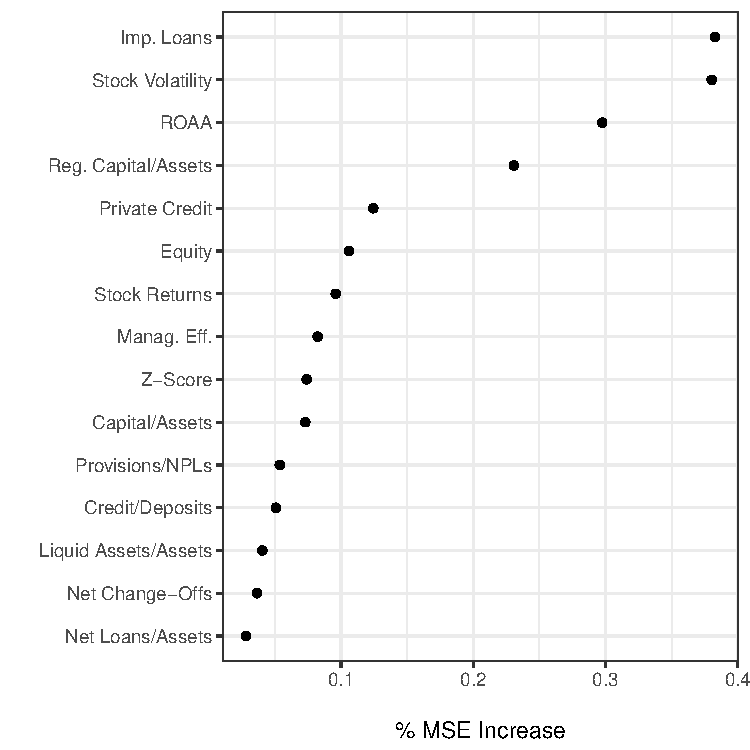
\includegraphics[scale=0.5]{figures/rf_variable_imp.pdf}
    \end{center}
\end{figure}

\begin{landscape}
\begin{figure}
    \caption{Partial Dependence of Each Predictor in the Random Forest Regression on FinStress ($\hat{y}$)}
    \label{rf_partial_depend}
    \begin{center}
        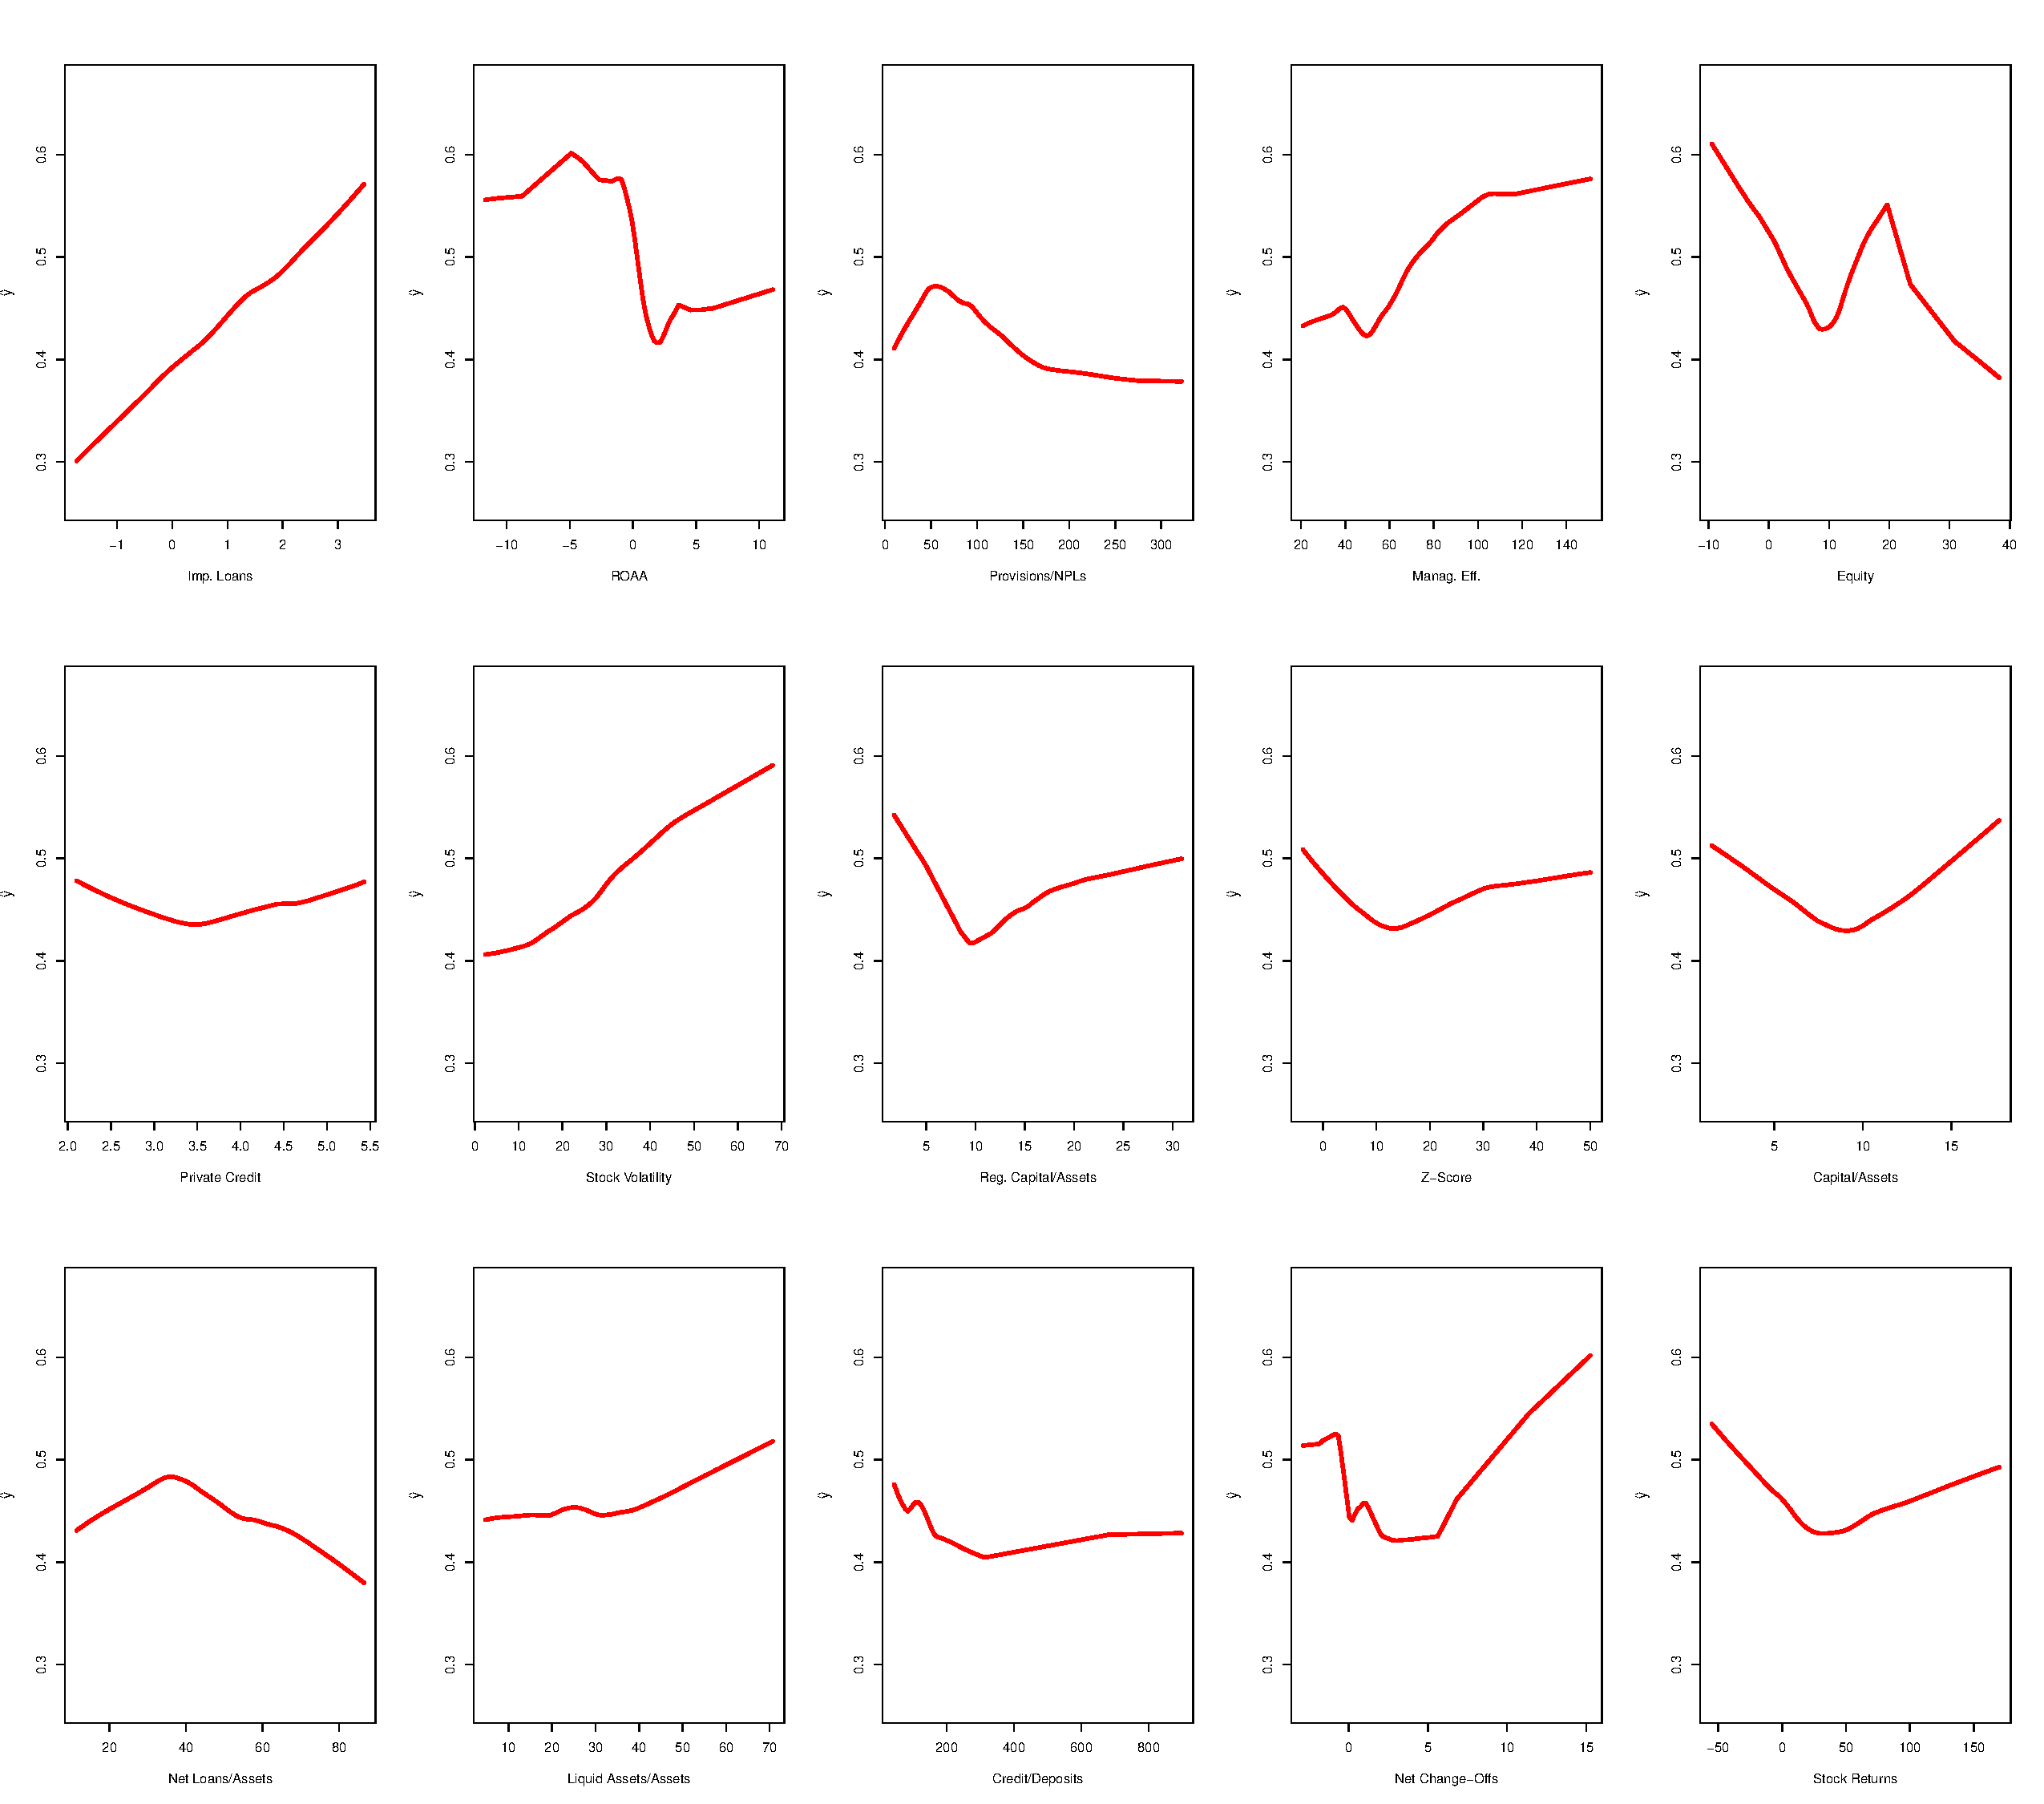
\includegraphics[scale=0.42]{figures/rf_partial_dependence.pdf}
    \end{center}

\end{figure}
\end{landscape}

\section{Conclusions}\label{conclusions}

We have introduced a novel continuous measure of real-time perceived financial, specifically banking market stress--FinStress--and compared it to prior measures of financial stress and crisis. Unlike previous measures of extreme stress--crises--, FinStress does not focus exclusively on financial market difficulties that, in hindsight, were not dealt with effectively by policymakers. This could allow future researchers to examine what policies were effective at preventing full blown crises and what political conditions were conducive to implementing these policies. Being an indicator of perceived and real-time stress, rather than a \emph{post hoc} evaluation of policy decisions in response to market events, FinStress provides a much more relevant indicator for understanding policymakers' decision-making processes. The measure also has considerably better coverage than previous quantitative measures of stress over the time period for which it is currently available. In sum, FinStress should be used instead of previous second-best measures of financial market stress by researchers aiming to understand why and how policymakers respond to the stress that they face in financial markets.

Our work has implications for the wider research community as well. We have demonstrated how researchers could construct continuous indicators of other political and economic phenomena using machine learning and text analysis. Once a text gathering and analysis ``pipeline'' \citep{Leek2015} has been developed and validated, researchers using this approach can quickly and cost effectively estimate and update new indicators. This approach is especially useful in comparison to time-consuming, expensive, and irreproducible human coding techniques.

\bibliographystyle{apsr}
\bibliography{main.bib}

\pagebreak
\renewcommand{\thepage}{A-\arabic{page}}\setcounter{page}{1}
\renewcommand{\thesection}{Appendix \arabic{section}}\setcounter{section}{0}
\renewcommand{\thetable}{A-\arabic{table}}\setcounter{table}{0}
\renewcommand{\thefigure}{A-\arabic{figure}}\setcounter{figure}{0}
\clearpage

\section*{Online Appendix}

\begin{table}[H]
    \caption{Comparison of Binary Crisis Measures' Definitions}
    \label{comp_table}
    \begin{center}
        \begin{tabular}{m{3cm} | m{2cm} m{2cm} m{7cm}}
            Source & Measurement Level & Periodicity &  Definition of Financial Market Distress/Crisis \\
            \hline\hline
                Reinhart and Rogoff \citeyearpar[11]{Reinhart2009,ReinhartRog2010} & binary & annual & One of two types of events: (1) bank runs leading to closures, mergers, or public sector takeovers of one or more financial institution or (2) the closure, merger, takeover, or large-scale government assistant--at least three measures--of an important financial institution marking the start of a string of similar events.  \\[1cm]
                Laeven and Valencia \citeyearpar[228]{laeven2013} & binary & annual & Meets two conditions: (1) significant sign of financial distress in the banking system and (2) significant banking policy intervention measures in response to significant losses in the banking system.  \\[1cm]
            \hline
        \end{tabular}
    \end{center}
\end{table}

\subsection*{Selection of Literature Including Binary Cross-Country Measures of Financial or Banking Market Crisis}

\begin{table}[H]
\caption{Selected Literature Review of Political Institutions and Financial
Crisis (Binary Crisis Occurrence, Political Outcomes)}


\label{LitRevTable2}
\begin{center}

\vspace{0.5cm}
{\tiny{
\begin{tabular}{ m{2.5cm} m{1.75cm} m{6.25cm} m{2.5cm} }
    \hline
    Work & Crisis Type & Key Arguments/Findings & Crisis Data Sources \\
    \hline\hline

    %%% Bernhard and Leblang
    \cite{Bernhard2008} & Currency crisis & - Changes in the probability that cabinets will collapse condition the probability of speculative attacks.

    - Higher probability of a speculative attack decreases the probability of calling strategic elections. & Own data aggregated from multiple sources \\[0.25cm]\hline

    %%% Chwieroth and Walter
    \cite{Chwieroth2013} & Banking crises &  - Probability of government survival during crises changed over time as expectations changed about what governments should do to respond.

    - Governments with more veto players after the inter-war period are treated more harshly by voters. & \cite{ReinhartRog2010} \\[0.25cm]\hline

    \cite{CrespoTenorio2014} & Banking crisis & - Increasing globalization weakens the accountability link between politicians and voters.

    - Incumbents in open capital economies are more likely to survive a crisis, than those in closed economies. & Own data aggregated from multiple sources. \\[0.25cm]\hline

    %%% Montinola
    \cite{Montinola2003} & Banking crisis & - IMF credits decrease the probability of resolving banking crises.

    - The decisiveness of a political regime significantly influences the probability of emerging from systemic distress, though this depends on whether the crisis is moderate or severe. & Own data aggregated from multiple sources \\[0.25cm]\hline

    %%% Pepinsky
    \cite{Pepinsky2012} & Banking crisis & - Two factors--incumbent governments' responsibility for the current crisis and their responsiveness to its domestic economic effects--shape the political effects of the global economic crisis. & \cite{Laeven2010} \\[0.25cm]\hline

    \hline
\end{tabular}

}}
\end{center}
\end{table}

\begin{table}[H]
\caption{Selected Literature Review of Political Institutions and Financial
Crisis (Binary Crisis Occurrence, Policy Choices/Policy Outcomes)}


\label{LitRevTable}
\begin{center}

\vspace{0.5cm}
{\tiny{
\begin{tabular}{ m{2.5cm} m{2cm} m{7cm} m{3cm}}
    \hline
    Work & Crisis Type & Key Arguments/Findings & Crisis Data Sources \\
    \hline\hline

    %%% Broz
    \cite{broz2013} & Banking crisis & - In OECD countries right-wing governments pursue policies that lead to financial instability. Voters respond to resulting crises by voting in left-wing governments. & \cite{Reinhart2009,Laeven2012} \\[0.25cm]\hline

    %%% Galasso
    \cite{galasso2014} & Financial and economic crises & - Governments respond to financial crises by increasing regulation. & Dummy based on OECD output gap below -3.4\% \\[0.25cm]\hline

    %%% Gandrud
    \cite{Gandrud2013,Gandrud2014} & Banking crises & - Best practice financial governance institutional designs are more likely to be adopted during crises when there is high uncertainty about policy choices and outcomes. & \cite{Laeven2008,ReinhartRog2010} \\[0.25cm]\hline

    %%% Ha and Kang
    \cite{ha2015} & - Banking crisis & Developing countries respond to crises with fiscal and monetary tightening, which was moderated by political constraints, left ideology governing parties, and up coming elections. & \cite{Laeven2008}. \\[0.25cm]\hline

    %%% Hallerberg Scart
    \cite{HallerbergScartForthcoming} & Banking, debt crises & - Banking crises reduce the probability of fiscal reforms, but the longer a crisis lasts and if it becomes a sovereign debt crisis the the probability of reform increases.

    - Countries with more personalistic voting are more likely to reform. & \cite{Laeven2012} for Latin American countries \\[0.25cm]\hline

    %%% Hallerberg Wehner
    \cite{Hallerberg2013} & Banking, currency, debt crises & - Some evidence that more technically competent ministers of finance are appointed during debt crises. Not much robust evidence for other effects of crisis on the technical competency of economic policy-makers. & \cite{Laeven2012}  \\[0.25cm]\hline

    %%% Hicken et al.
    \cite{Hicken2005} (2005) & Growth shocks & - The size of the winning coalition is positively associated with growth recoveries following forced devaluations. & Own data aggregated from multiple sources \\[0.25cm]\hline

    %%%% Keefer
    \cite{Keefer2007} & Banking crises & - Higher electoral competitiveness leads to faster and less costly crisis responses.

    - Checks and balances not associated with crisis policy choices or outcomes. & Modified \cite{Honohan2003} \\[0.25cm]\hline

    %%% Kleibl
    \cite{Kleibl2013} & Banking crisis & - Responses to regulatory failures are conditioned by the level of public ownership in the banking sector. & \cite{Laeven2010,Reinhart2009} for OECD countries \\[0.25cm]\hline

    %%% MacIntyre
    \cite{MacIntyre2001} & Financial crises & - U-shaped relationship between veto players and crisis outcomes & Own data aggregated from multiple sources \\[0.25cm]\hline

    %%% Reischmann
    \cite{reischmann2015} & Banking crises & - Creative accounting as measured by changes in the stock flow adjustment occurs more during financial crises, though effect may be swallowed up by the period fixed effects in his regressions as crises are highly correlated with time in his sample. & \cite{Laeven2012} \\[0.25cm]\hline

    %%% Rodrick
    \cite{Rodrick1999} & Growth shock & - Many veto players, if organized to manage conflicts, will result in more appropriate and quickly implemented crisis management policies. & Own data aggregated from multiple sources \\[0.25cm]\hline

    %%%% Rosas
    \cite{Rosas2006,Rosas2009} & Banking crisis & - Democratic regimes have fewer bailouts.

    - Central bank independence and transparency lead to fewer bailouts. & Modified \cite{Honohan2000} \\[0.25cm]\hline

    %%% Seiferling and Tareq
    \cite{seiferling2015} & Banking crisis & - Find advanced economies governments extend more loans and purchase more equities in temporarily insolvent firms during financial crisis than emerging market governments. & \cite{Laeven2010} via \cite{weber2012} \\[0.25cm]\hline

    %%% Satyanath
    \cite{Satayanath2006} & Banking crises & - Executives without `banking cronies' and that are not prevented from appointing their own bureaucrats by many veto players are more likely to have stringent financial regulation that prevents crises. & Case studies of 7 East Asian countries using own data \\[0.25cm]\hline

    %%% Wibbels and Roberts
    \cite{Wibbels2010} & Currency, growth, \& fiscal crises & - Unions and strong left parties are more associated with crises, though combined strong unions-left parties may alleviate inflationary crises. & Own data aggregated from multiple sources for 17 Latin American countries \\[0.25cm]\hline


    \hline
\end{tabular}

}}
\end{center}
\end{table}

\subsection*{Developed vs.~developing
countries}\label{developed-vs.developing-countries}

Developing countries often lack strong financial institutions and systems. Facing a very risky pool of borrowers, banks tend to make fewer loans \citep{Andrianova2014}. So we should expect them to face generally tighter credit market conditions than developed countries.

The left panel of Figure \ref{comp_dev_developing} shows average stress levels in developed vs. developing countries that Laeven and Valencia code as not being in crisis--indicates that there is a difference in the level of perceived financial market stress in developed and developing countries from 2003 to 2008. Developing countries on average have higher FinStress scores. For example, the mean score in middle and low income countries (as classified by the World Bank) is 0.53 in 2005, a level developed countries only reached after the collapse of Lehman Brothers in 2008.\footnote{The 2005 mean for high income countries is 0.44} The mean levels across the two groups converge in the Global Financial Crisis. The distribution of FinStress scores in these two groups of countries across the sample is significantly different in the expected direction in the sample using one-sided Kolmogorov-Smirnov tests.\footnote{We ran the tests using the \texttt{ks.test} function from base R.}

Nonetheless, during periods when the binary Laeven and Valencia code as being a crisis, i.e. implement policy responses to financial market stress,the two sets of scores are very similar (see the right-panel of Figure \ref{comp_dev_developing}). Apart from 2007 and 2008 where the binary measures have significant ``annual rounding error'',\footnote{They include both less and more stressed portions of a year as a crisis} on average countries in crisis have FinStress scores above about 0.55. It appears that while developed countries have more stressed financial markets than developed countries that on average, developed and developing countries have clear policy responses to financial market stress when their FinStress scores are above about 0.55.

\begin{figure}
    \caption{Comparison of Mean FinStress Scores in High vs. Low and Medium Income Countries}
    \label{comp_dev_developing}

    \begin{center}
        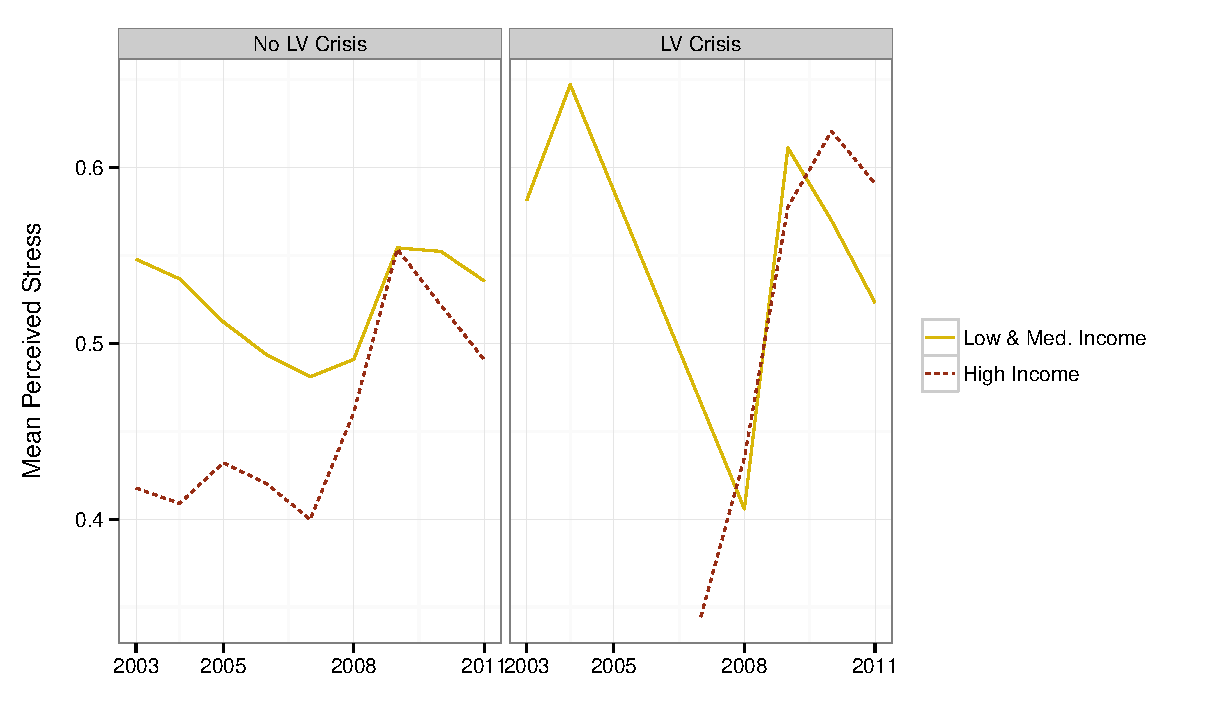
\includegraphics[scale=0.55]{figures/dev_vs_developing.pdf}
    \end{center}
    {\scriptsize{Plot excludes Uruguay, which was a substantial outlier with a much lower average FinStress score during what Laeven and Valencia classify as a crisis than all other developing countries.}}
\end{figure}

\subsection*{Correlations Between FinStress and Camel Variables}

\begin{figure}[H]
	\caption{Correlation between Annual FinStress Mean Scores and CAMELS Variables from \cite{Andrianova2015}}
    \label{cor_camel}
    \begin{center}
    	\includegraphics[scale=0.5]{figures/ff_corr_matrix.pdf}
    \end{center}
\end{figure}

\subsection*{FinStress compared to Z-Scores}

How does FinStress compare to the widely used Z-Score measure of banking system fragility? We saw in the main text that the global random forest regression indicates that Z-Scores are not very predictive of FinStress. Given the prominence of the Z-Score measure in the finance literature, we wanted to further explore this (none) relationship.

It is important to note that the two quantities do measure different phenomena--perceptions for the former and bank accounting relationships for the latter--both potentially  provide indications of stress. As was the case for the dichotomous measures of financial crises, we would expect them to be positively correlated with one another. Another interesting question would be whether one would precede the other. Does weakness in accounting quantities proceed perceived stress?

To explore these possibilities, we compare FinStress to the easily accessible Bank Z-Score measure compiled from Bankscope data in the World Bank's Global Financial Development Database (GFDD) project \citep{worldbank2013}.\footnote{Indicator ID: GFDD.SI.01. Accessed June 2015.} The measure is interpretable as the inverse of the upper bound of the probability of the banking system's insolvency.\footnote{Formally: $\frac{\mathrm{ROA}_{t} + \frac{\mathrm{equity}_{t}}{\mathrm{assets}_{t}}}{\sigma_{\mathrm{ROA}}}$. $\mathrm{ROA}$ is return on equity. $\sigma_{\mathrm{ROA}}$ is presumably for the entire period for which data is available, though the World Bank's documentation does not explicitly specify this. It is common in other work for the $\sigma_{\mathrm{ROA}}$ to be based on a three year rolling window \cite[225]{beck2013bank}. All quantities are country aggregates.} Figure~\ref{z_score} shows a comparison of the two measures for selected countries. Note that to ease visual comparability we rescaled the Z-Scores to be within zero and one as before, and reversed the scale so that larger values indicate a higher probability of banking system insolvency.\footnote{It is common to log-transform the Z-Scores \cite[225]{beck2013bank}. However, it is unclear how previous work has done this as there are negative values in the Z-score that would create undefined values when logged.} As before, we converted FinStress to yearly averages for comparability.

There does not appear to be much of a relationship between Z-Scores and FinStress. The rescaled World Bank Z-Scores are positively correlated with FinStress, but this is not significant at the 10\% level.\footnote{We also examined an alternative data source compiled by \cite{Andrianova2015}, which transformed Bankscope data as well. In this case there was a weak positive association significant at the 5\% level. However, again there was little cross-time variation in the Z-Score.} Interestingly, the World Bank's Z-Scores do not vary significantly within countries over time, especially compared to  FinStress. There is little difference between Z-Scores for countries during periods of heightened financial stress (however measured) and more stable times. Thus Z-Scores, at least those provided by the World Bank, are not a useful indicator of financial crisis states. Z-Scores do not appear to predict perceptions of financial market stress. In a simple partial correction linear regression that had FinStress as the dependent variable and included lagged FinStress, lagged Z-Scores, and country fixed-effects, Z-Scores were not statistically significantly associated with perceptions of financial market stress (see Table \ref{finstress_z_regress}).

The simplicity with which Z-Scores can be calculated with readily available data likely contributes to their wide use in the literature, especially relative to other quantitative measures of financial system fragility that are often difficult to obtain. However, it is clear that Z-Scores--at least the version available through the World Bank's GFDD--are a sub-optimal cross-time measure of financial market stress. It is beyond the scope of our article to determine the source of the measure's peculiar characteristics, but they are important to note here: the indicator has weak time-variance, it does not distinguish between periods of significant known financial market stress and less stressful times, and it does not help us predict perceived financial market stress. FinStress, in contrast, is much notably time-variant in ways that correspond closely to prior information on financial market stress.

\begin{figure}

    \caption{Annual Mean FinStress Compared to Country-level Z-Scores (rescaled)}
    \label{z_score}

    \begin{center}
        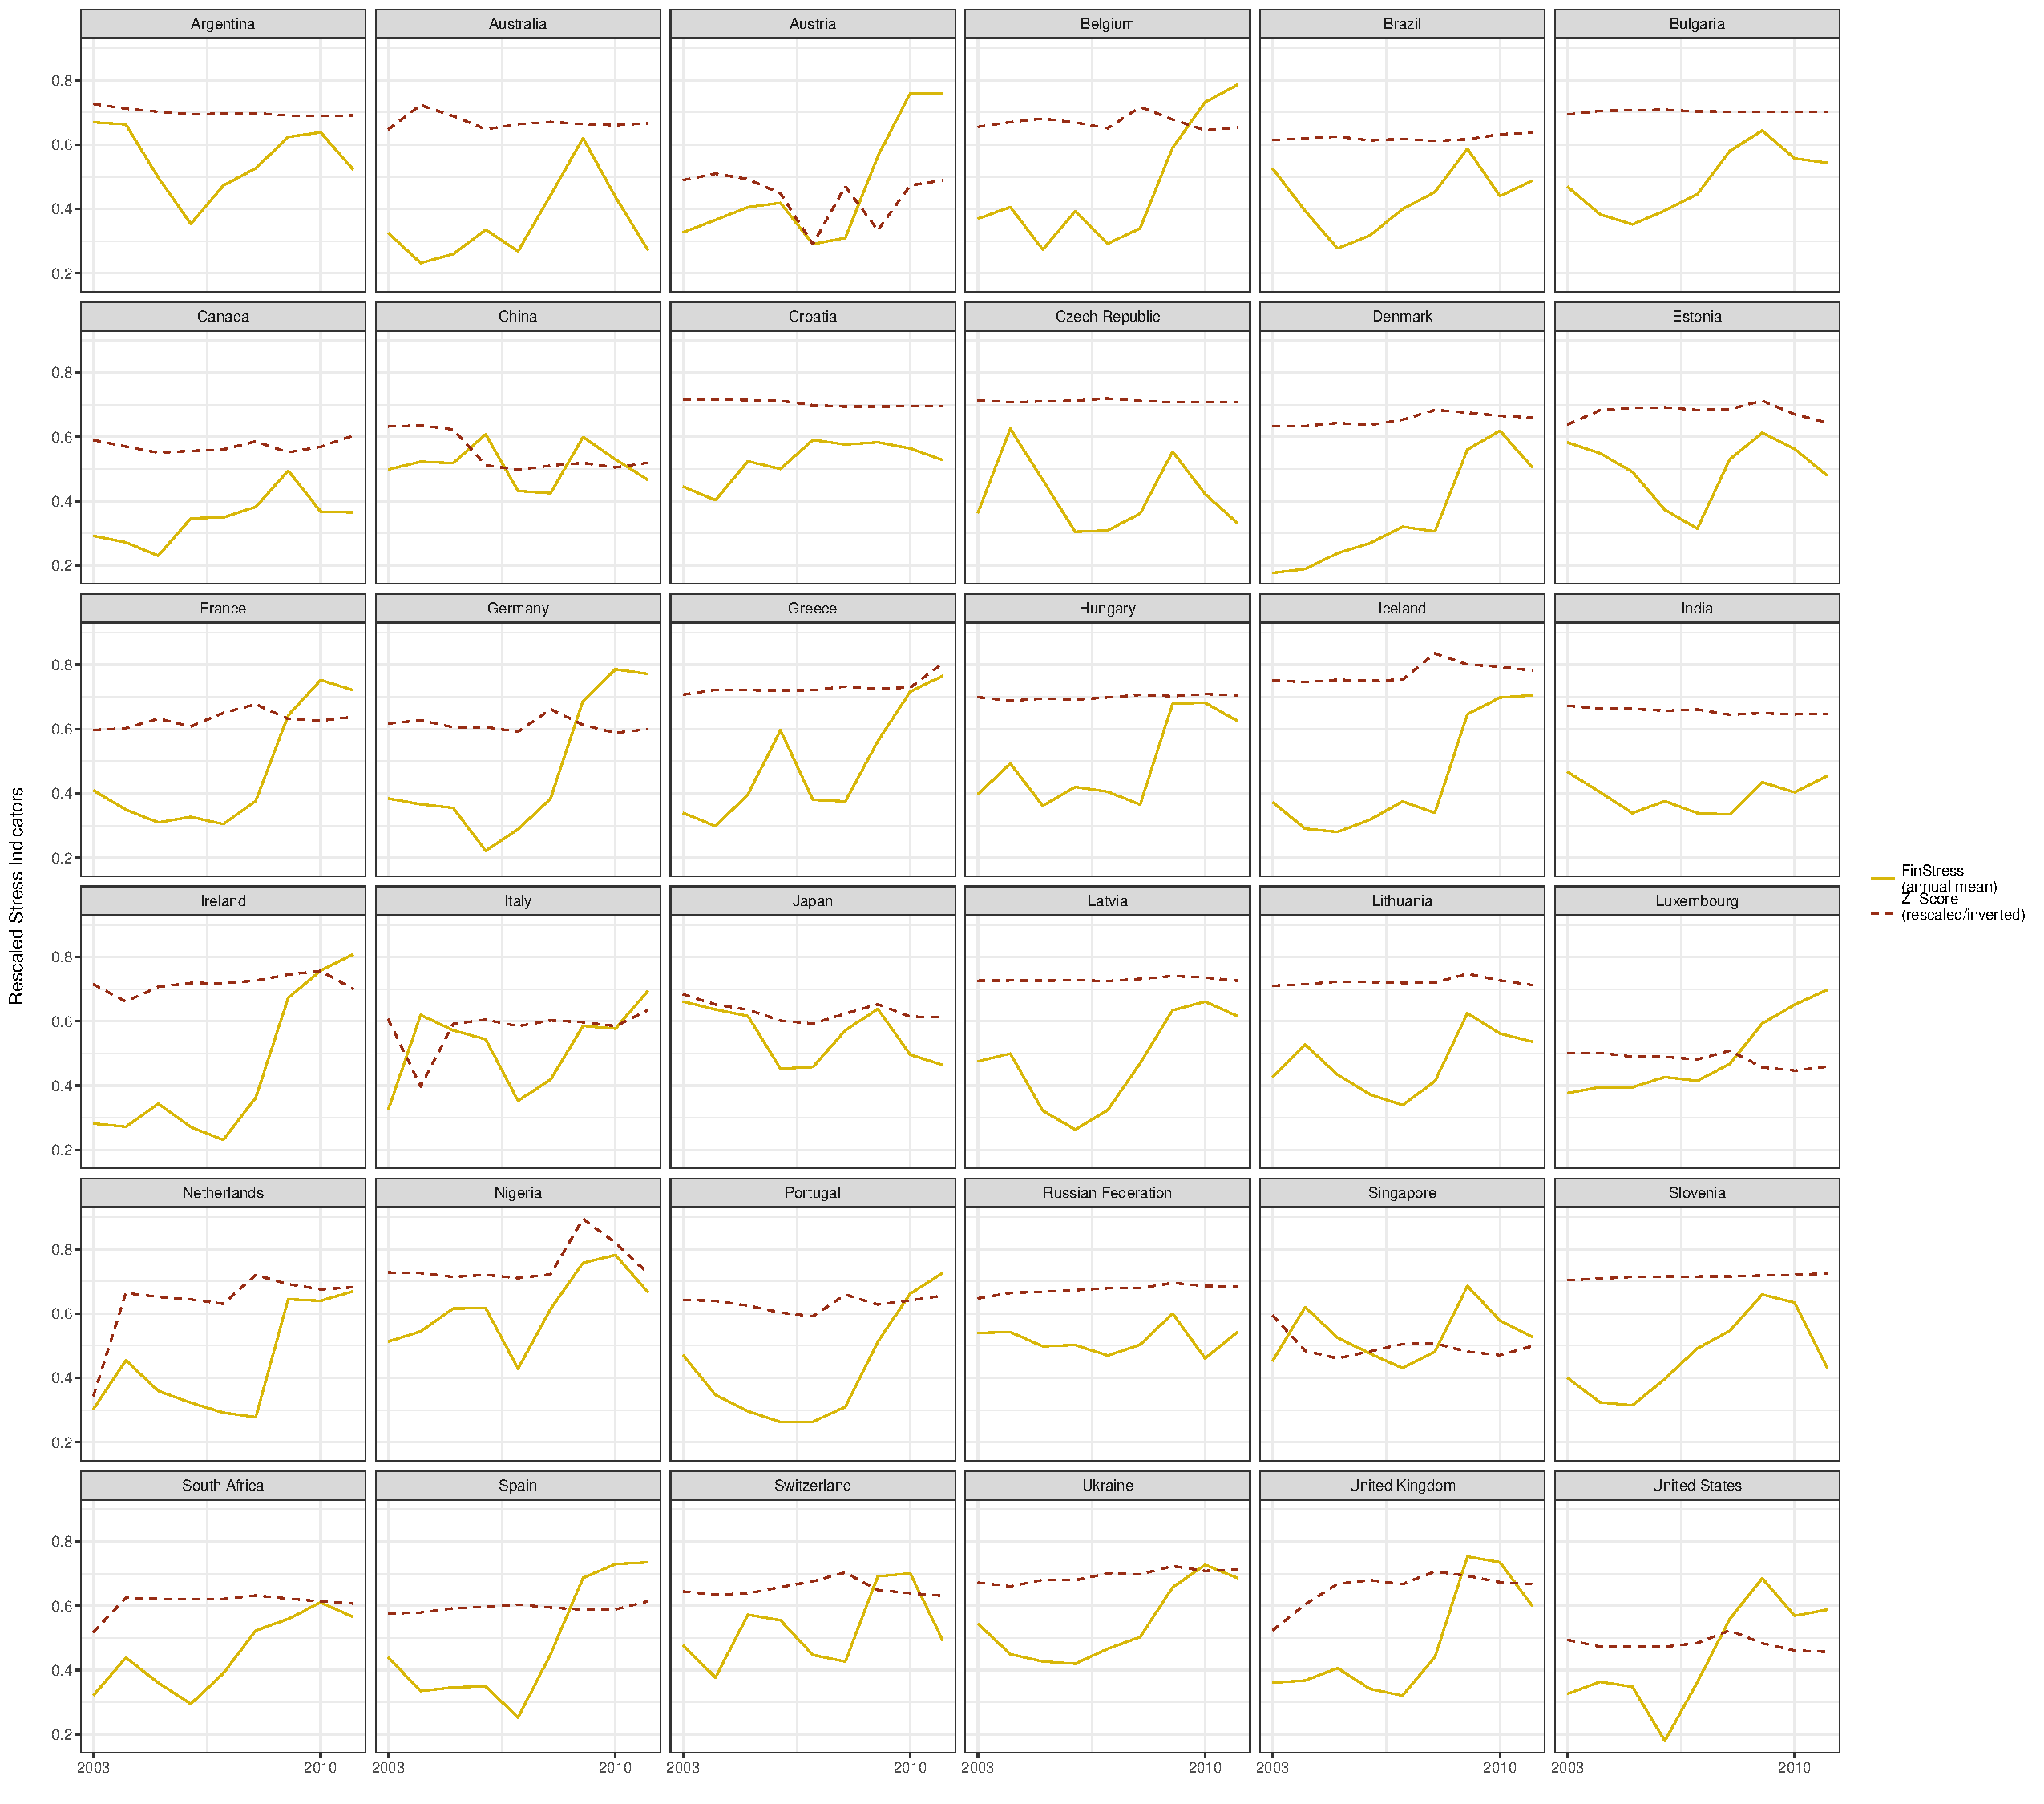
\includegraphics[scale=0.4]{figures/compare_to_z-score.pdf}
    \end{center}

\end{figure}

\begin{table}[H]
    \caption{Do Z-Scores Predict Perceived Financial Market Stress?}
    \label{finstress_z_regress}

    \begin{center}
    {\tiny{
        
% Table created by stargazer v.5.1 by Marek Hlavac, Harvard University. E-mail: hlavac at fas.harvard.edu
% Date and time: Mon, Jul 13, 2015 - 11:07:38
\begin{tabular}{@{\extracolsep{5pt}}lc} 
\\[-1.8ex]\hline 
\hline \\[-1.8ex] 
 & \multicolumn{1}{c}{\textit{Dependent variable:}} \\ 
\cline{2-2} 
\\[-1.8ex] & Annual Mean EPFMS \\ 
\hline \\[-1.8ex] 
 Annual Mean EPFMS (lag) & 0.339$^{***}$ \\ 
  & (0.023) \\ 
  & \\ 
 Z-Score (lag) & 0.0002 \\ 
  & (0.0004) \\ 
  & \\ 
\hline \\[-1.8ex] 
Fixed effects? & Yes \\ 
Observations & 1,464 \\ 
R$^{2}$ & 0.149 \\ 
Adjusted R$^{2}$ & 0.130 \\ 
F Statistic & 112.040$^{***}$ (df = 2; 1278) \\ 
\hline 
\hline \\[-1.8ex] 
\textit{Note:}  & \multicolumn{1}{r}{$^{*}$p$<$0.1; $^{**}$p$<$0.05; $^{***}$p$<$0.01} \\ 
\end{tabular} 

    }}
    \end{center}
\end{table}

\end{document}
